%====================================================================================================
% ?????
%====================================================================================================
% TCC
%----------------------------------------------------------------------------------------------------
% Autor				: Jasane Schio
% Orientador		: Gedson Faria
% Co-Orientador		: Angelo Darcy
% Instituição 		: UFMS - Universidade Federal do Mato Grosso do Sul
% Departamento		: CPCX - Sistema de Informação
%----------------------------------------------------------------------------------------------------
% Data de criação	: 01 de Outubro de 2015
%====================================================================================================
% NO FUTURO
\chapter{Resultados} 


	Para serem feitos os testes foram despostos no campo tiras coloridas entre 17 e 40 centimetros de largura e  5,5 e 10,5 centimetros de altura. Cada cor possue três tiras, e cada uma das tiras foi colocada em uma parte do campo que foi dividio em três.


Para a execução dos tipos de testes, o campo foi dividido verticalmente em cinco partes, de vinte e nove centimetros cada, e horizontalmente em três parte de quarenta e um centimetro cada, somando um total de quinze areas de calibração, nomeadas alfabeticamente de A à O, como mostrado na Figura \ref{campodivisao}.

\begin{figure}[!: h]
		\centering
		\includegraphics[width=0.3\textwidth]{campodivisao.pdf}
		\caption{Divisao do campo em quinze partes nomeadas alfabeticamente.}
		\label{campodivisao}
	\end{figure}
	
Em cada areas de calbração estão dispostas cinco cores: Vermelho  e Verde na primeira linha, Amarelo, Azul e Laranja na segunda. As cores estão distantes verticalmente \textit{7.5cm}, na primeria linha a distancia entre as cores é  de \textit{11 cm} e na segunda linha de \textit{7.2 cm}. Um  melhor detalhamento da disposiçao das cores é  mostrado na Figura \ref{disposicaoparte}. No total estavam disposto no campo quinze pontos de cada cor.


MUDAR ESSA FIGRURA
%\begin{figure}[H]
%		\centering
%		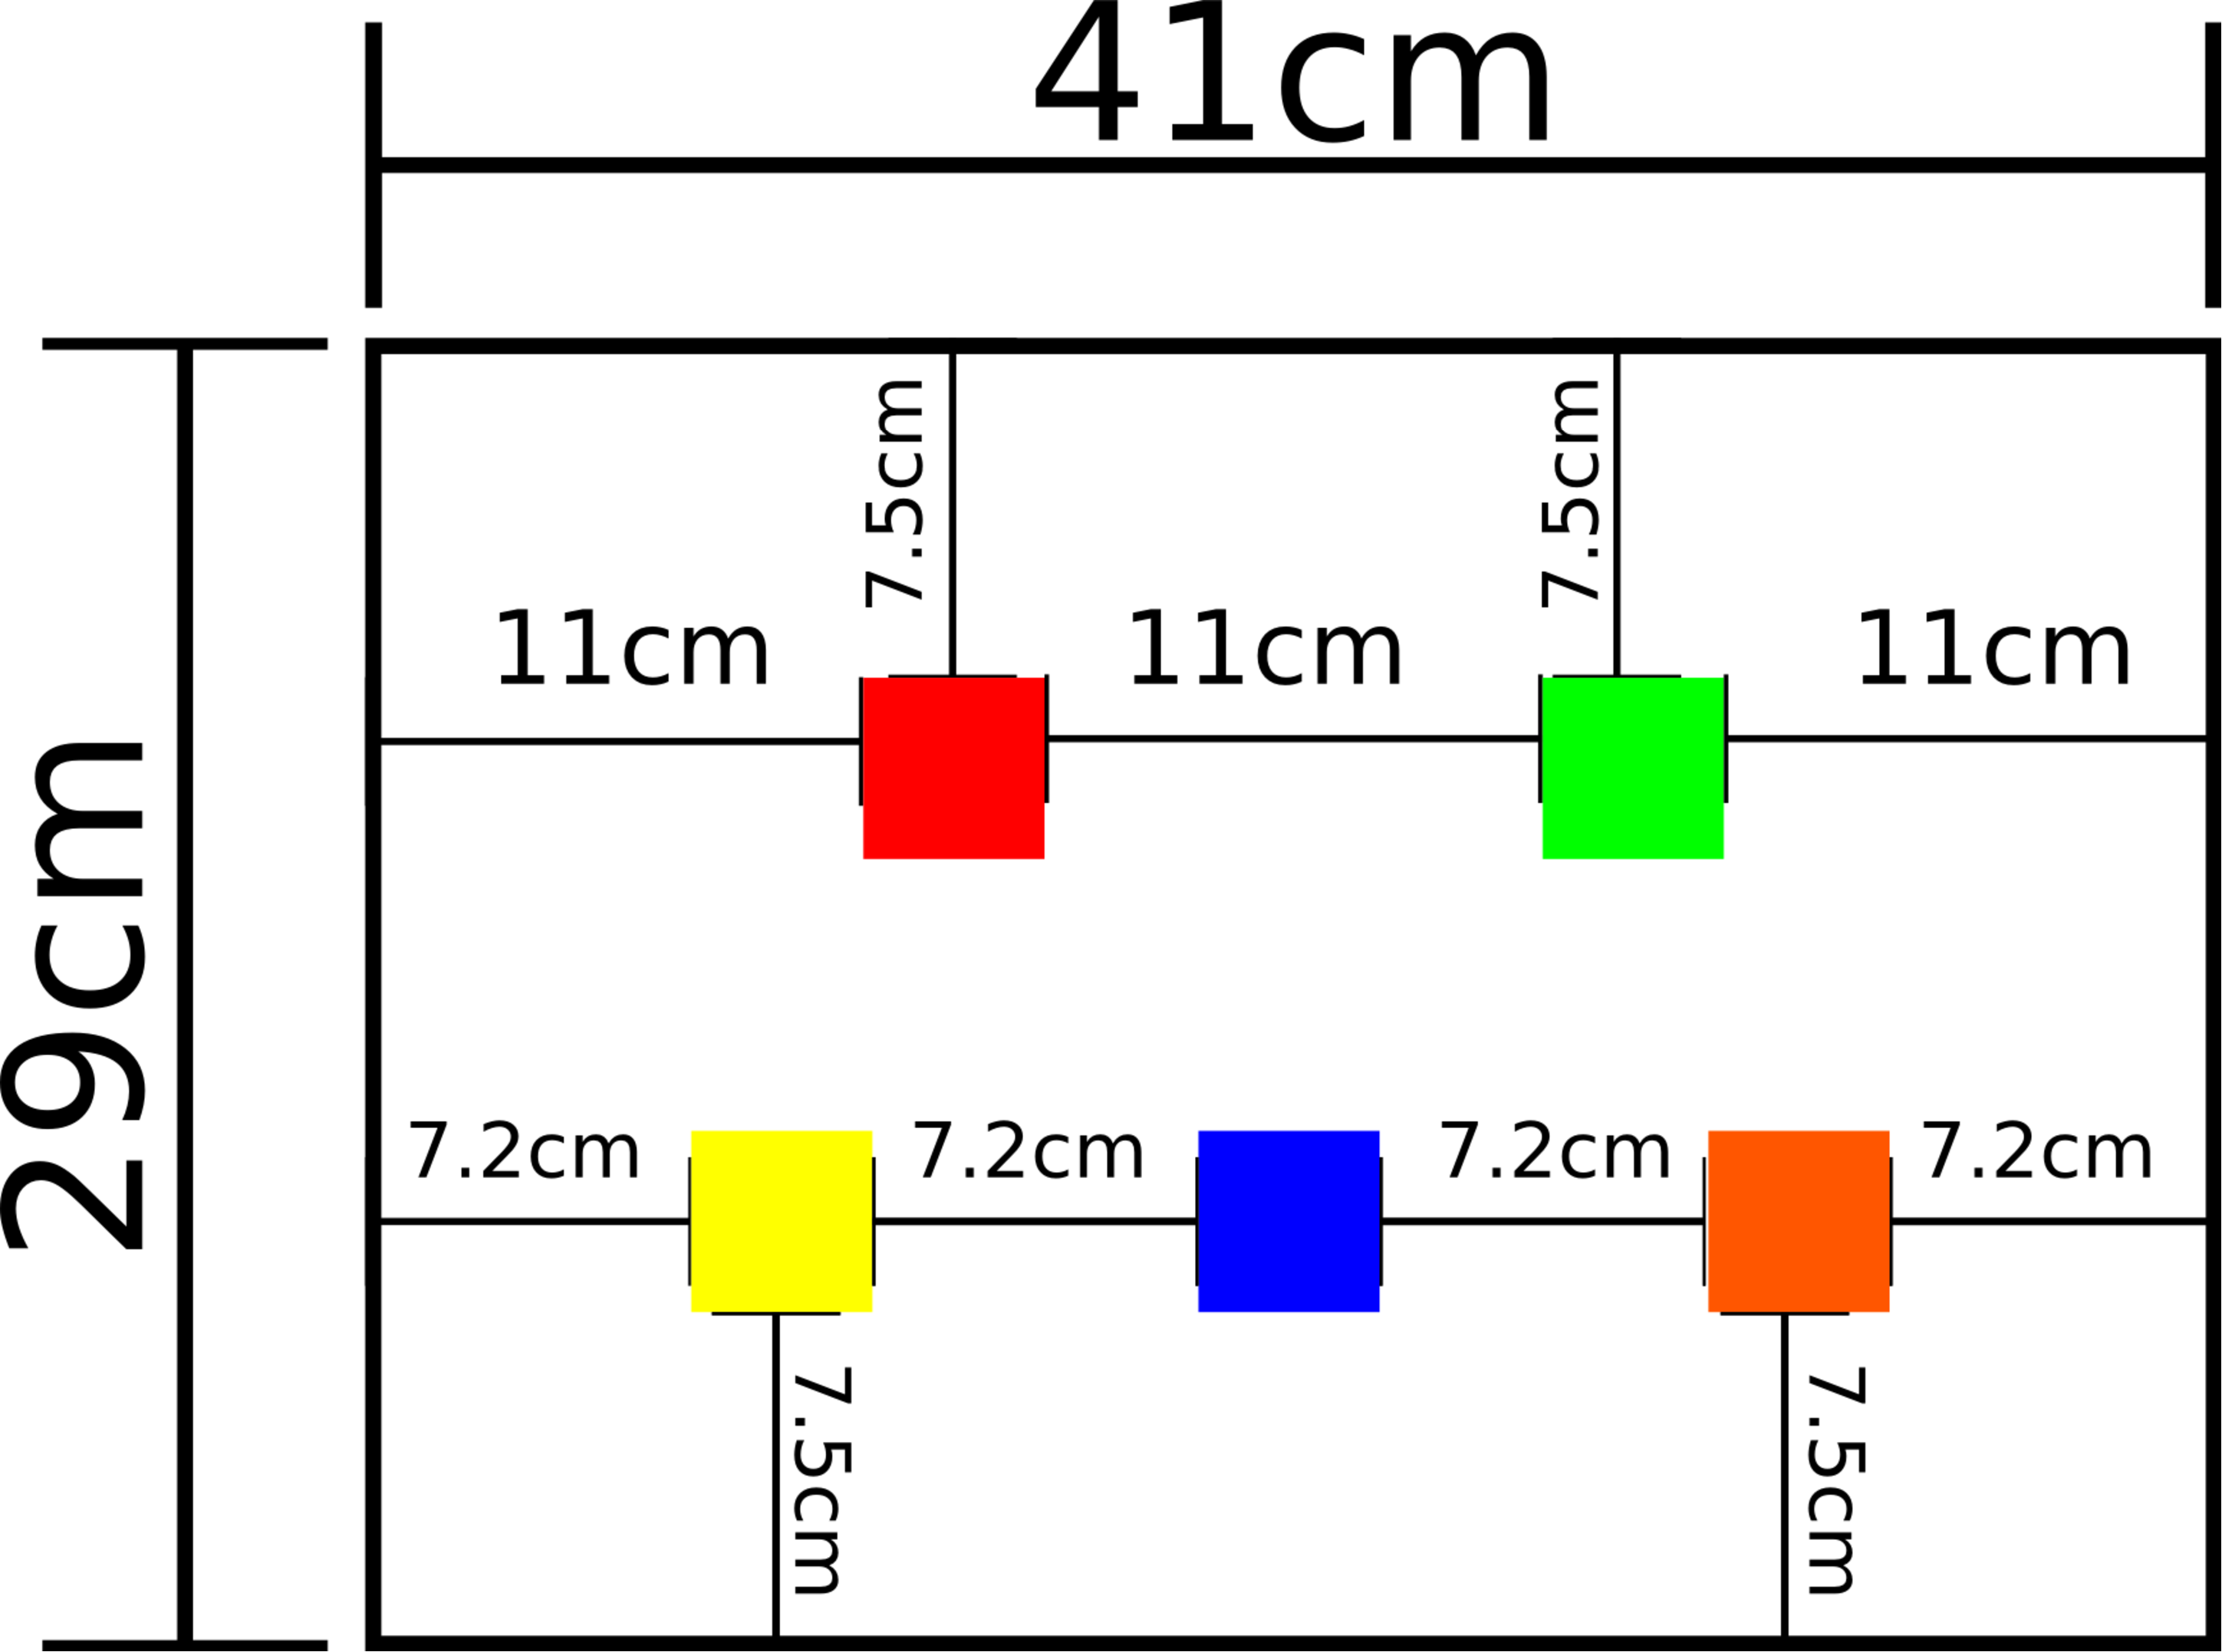
\includegraphics[width=0.3\textwidth]{disposicaoparte.pdf}
%		\caption{Disposição dos objetos coloridos dentro de cada uma das partes}
%		\label{disposicaoparte}
%	\end{figure}
\begin{figure}[H]
\begin{minipage}[b]{0.45\linewidth}
\centering
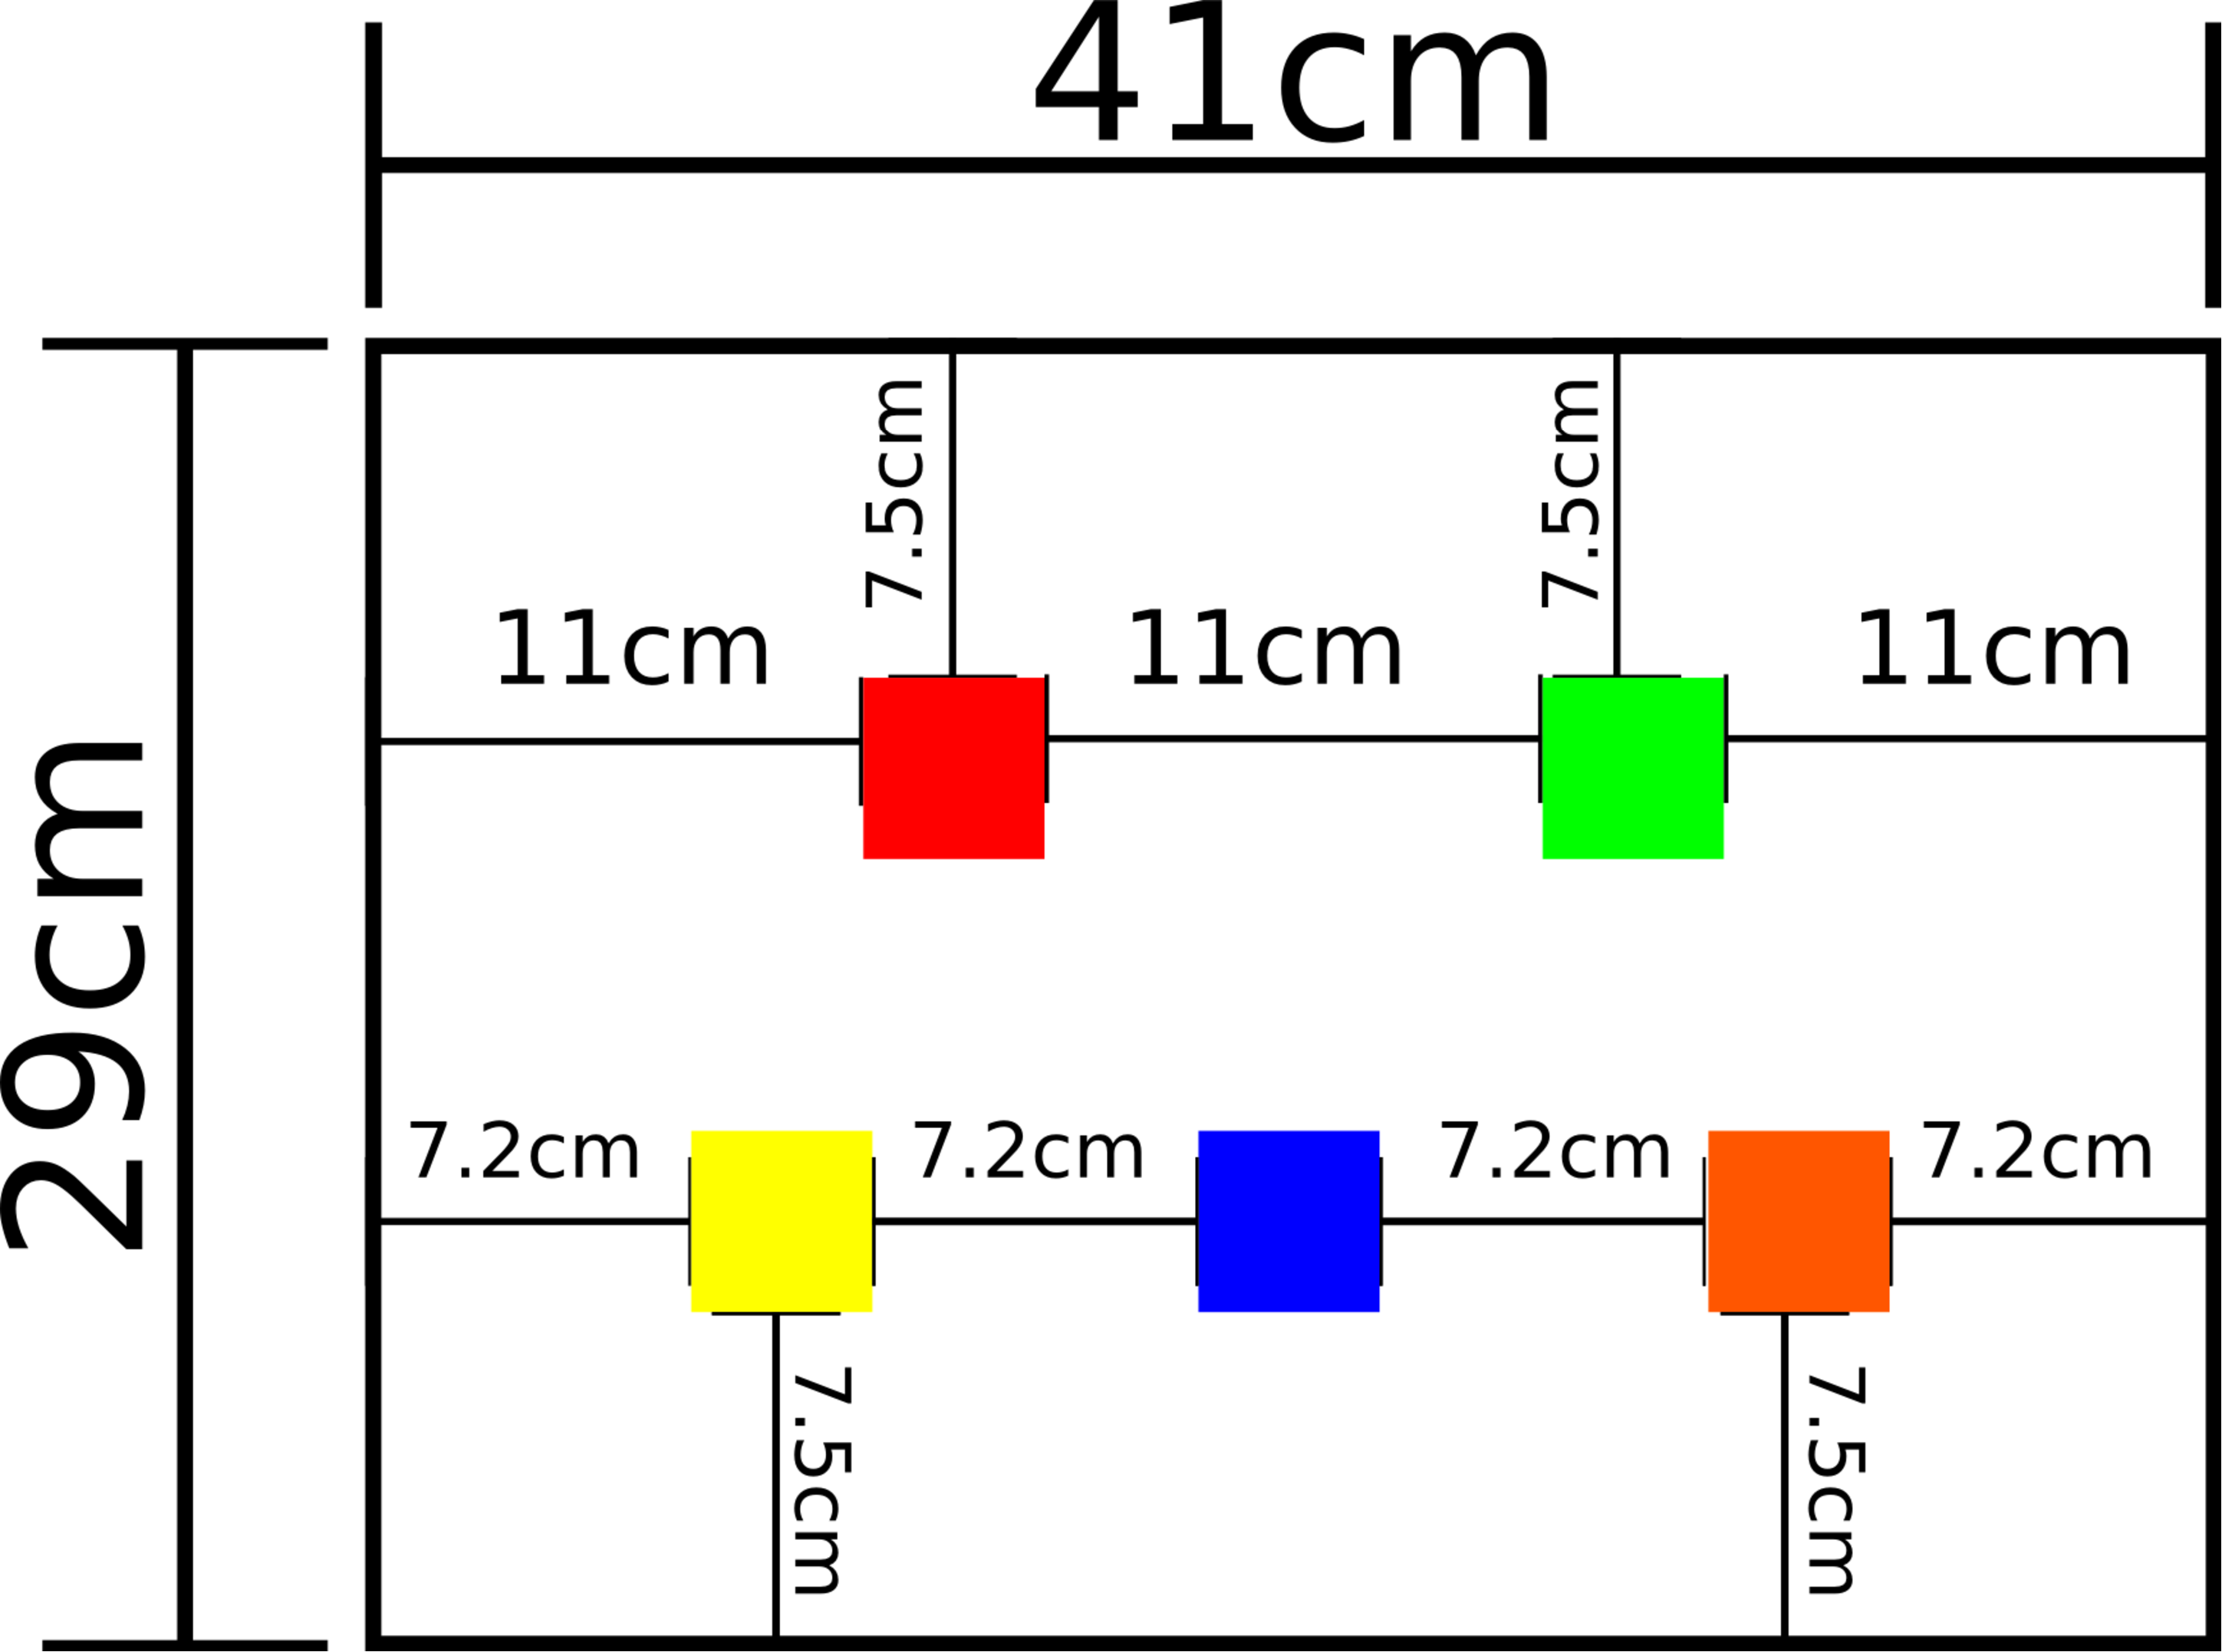
\includegraphics[width=\textwidth]{disposicaoparte.pdf}
\caption{Disposiçao de cada parte quanto as cores}
\label{fig:figure1}
\end{minipage}
\hspace{0.5cm}
\begin{minipage}[b]{0.45\linewidth}
\centering
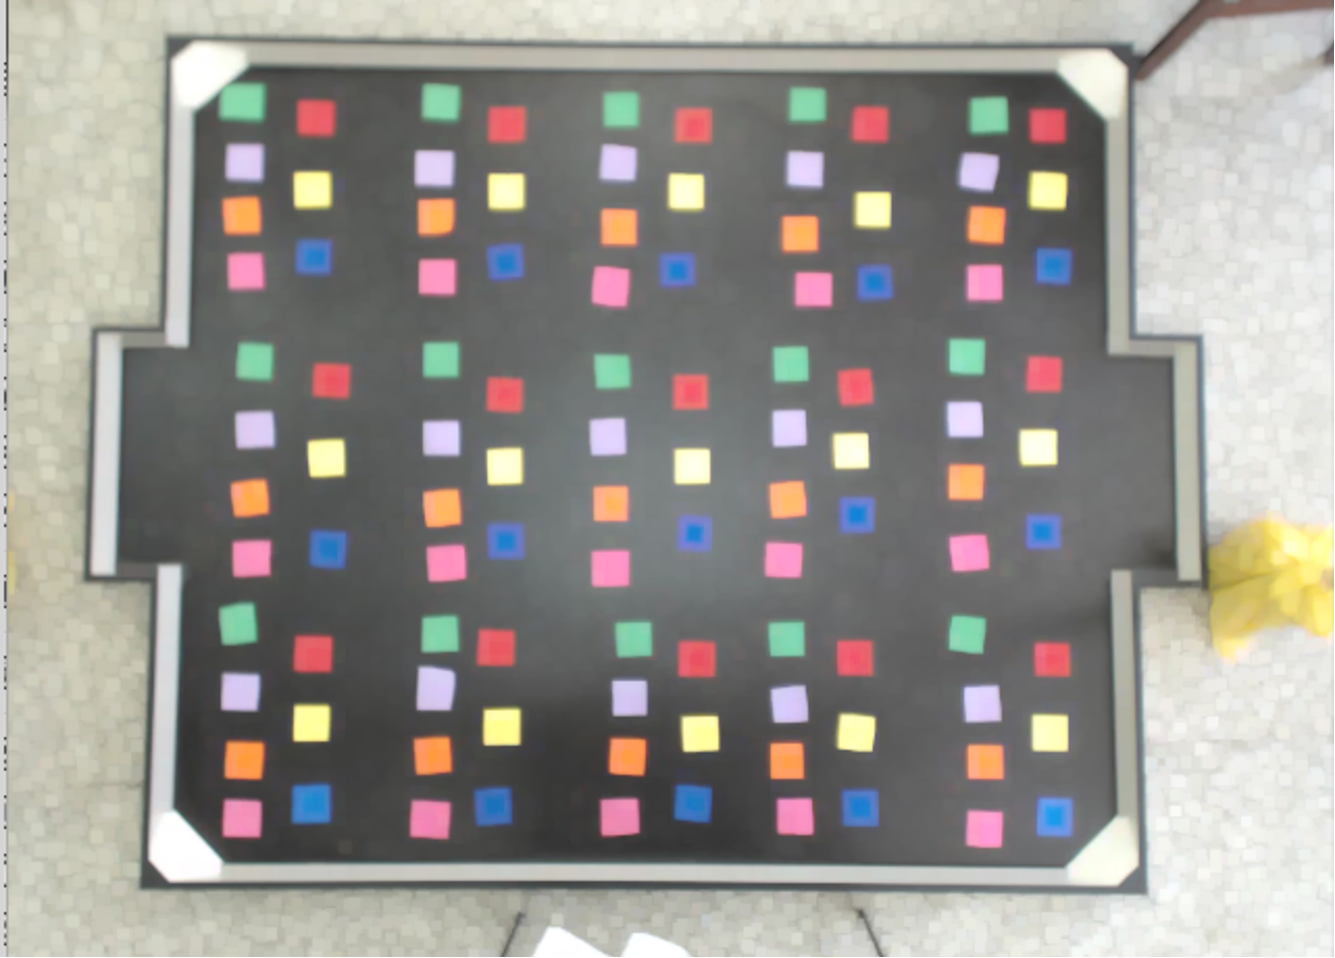
\includegraphics[width=\textwidth]{/testes/campofundo.pdf}
\caption{Campo apos terem sido dispostas as cores}
\label{fig:figure2}
\end{minipage}
\end{figure}

	
A realização da aquisição de minimos ocorreu dia 19 de Agosto de 2016, entre 17:36 e 17:39.

Seleção de Campo:
\begin{figure}[H]
		\centering
		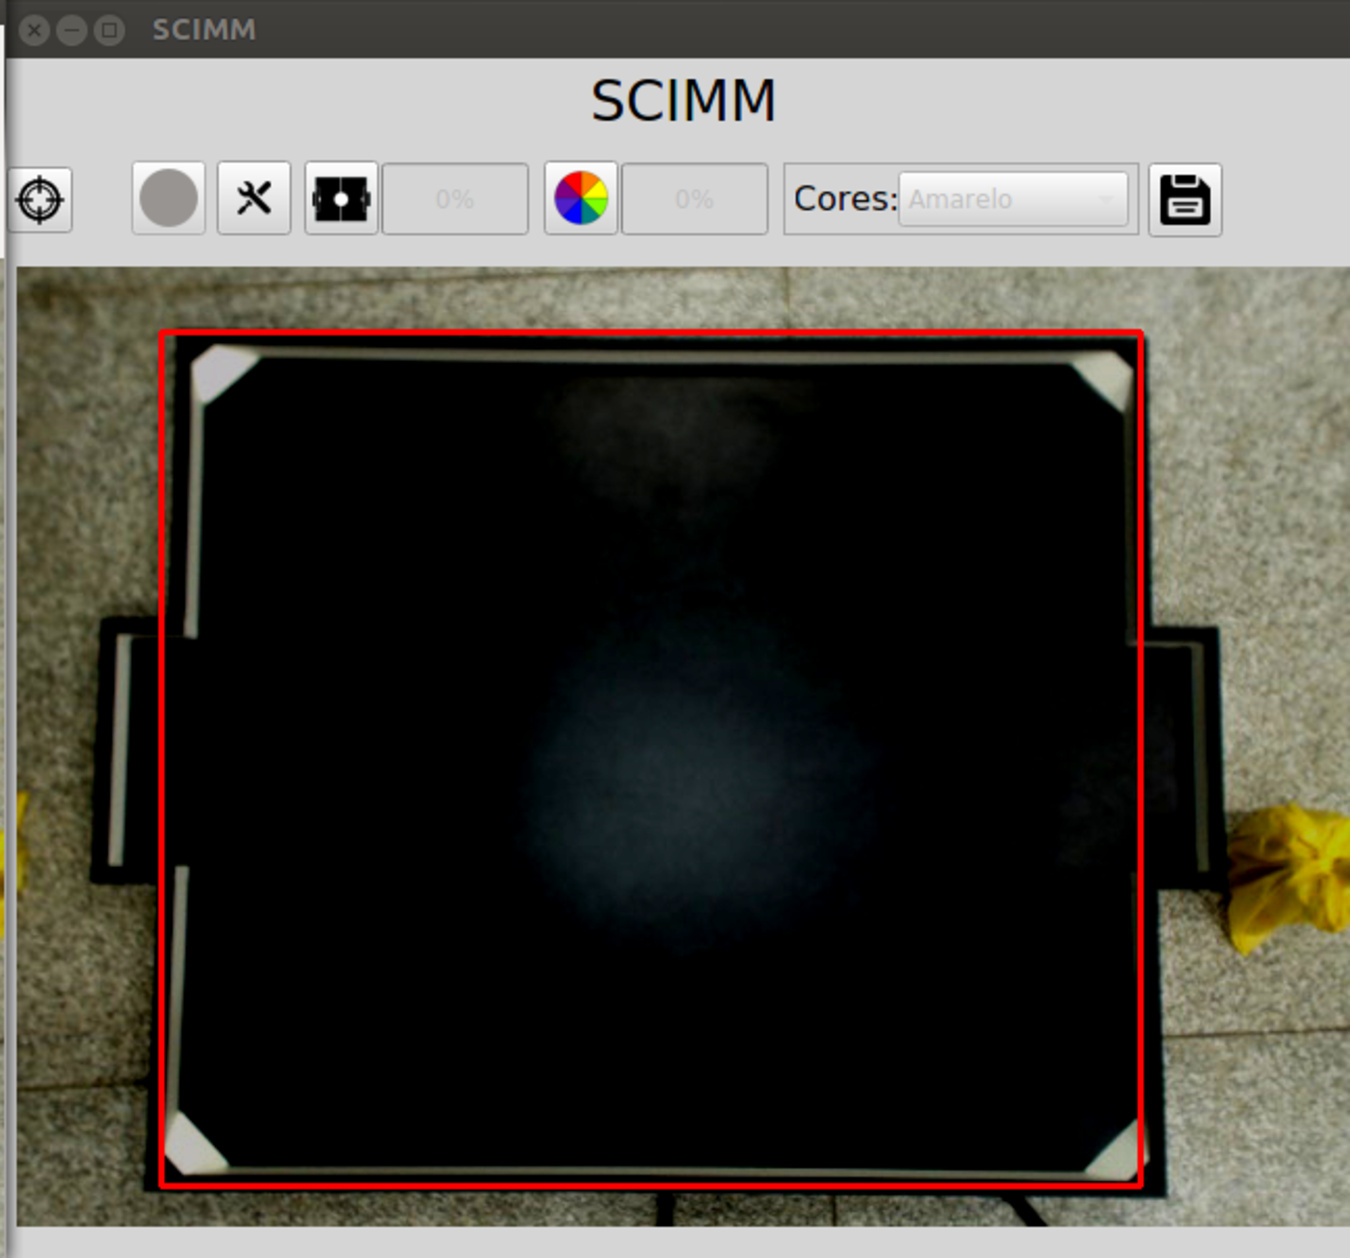
\includegraphics[width=0.6\textwidth]{fundoteste.pdf}
		\caption{Imagem do fundo com a seleção de campo}
		\label{disposicaoparte}
	\end{figure}
	
I%magem dos objetos dispostos:
%	\begin{figure}[H]
%	\centering
%		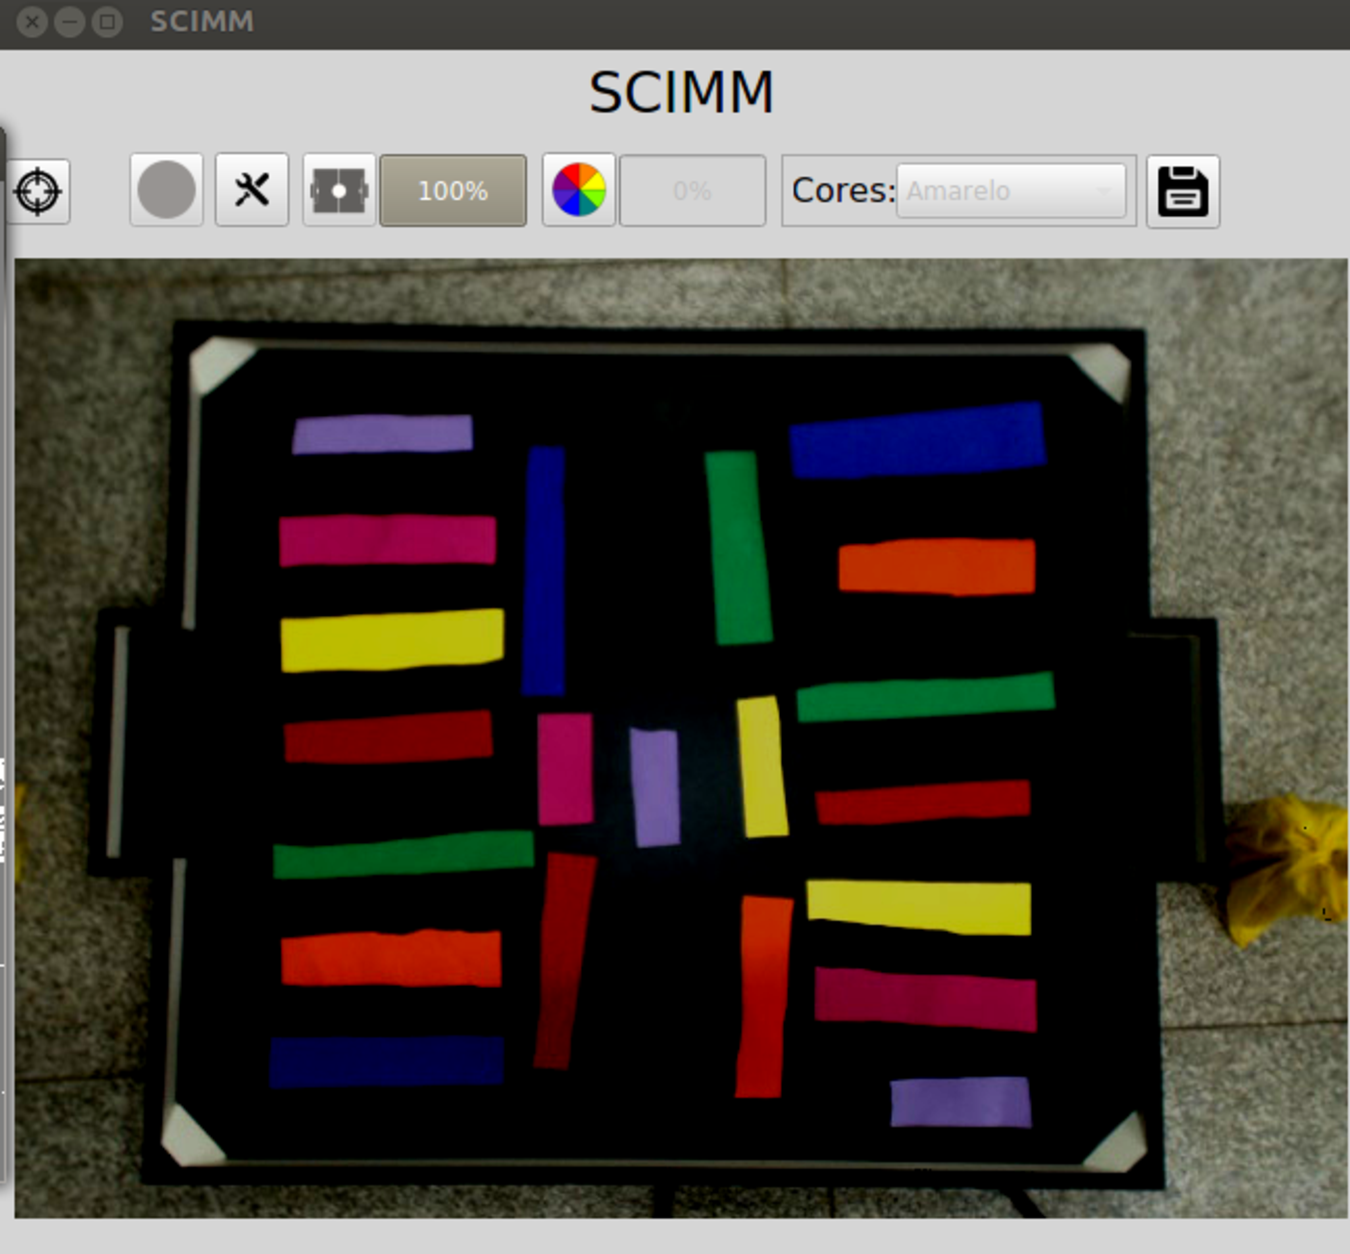
\includegraphics[width=0.6\textwidth]{objetosdispostos.pdf}
%		\caption{Objetos dispostos no campo para calibração}
%		\label{disposicaoparte}
%	\end{figure}
%	\begin{figure}[H]
%		\centering
%		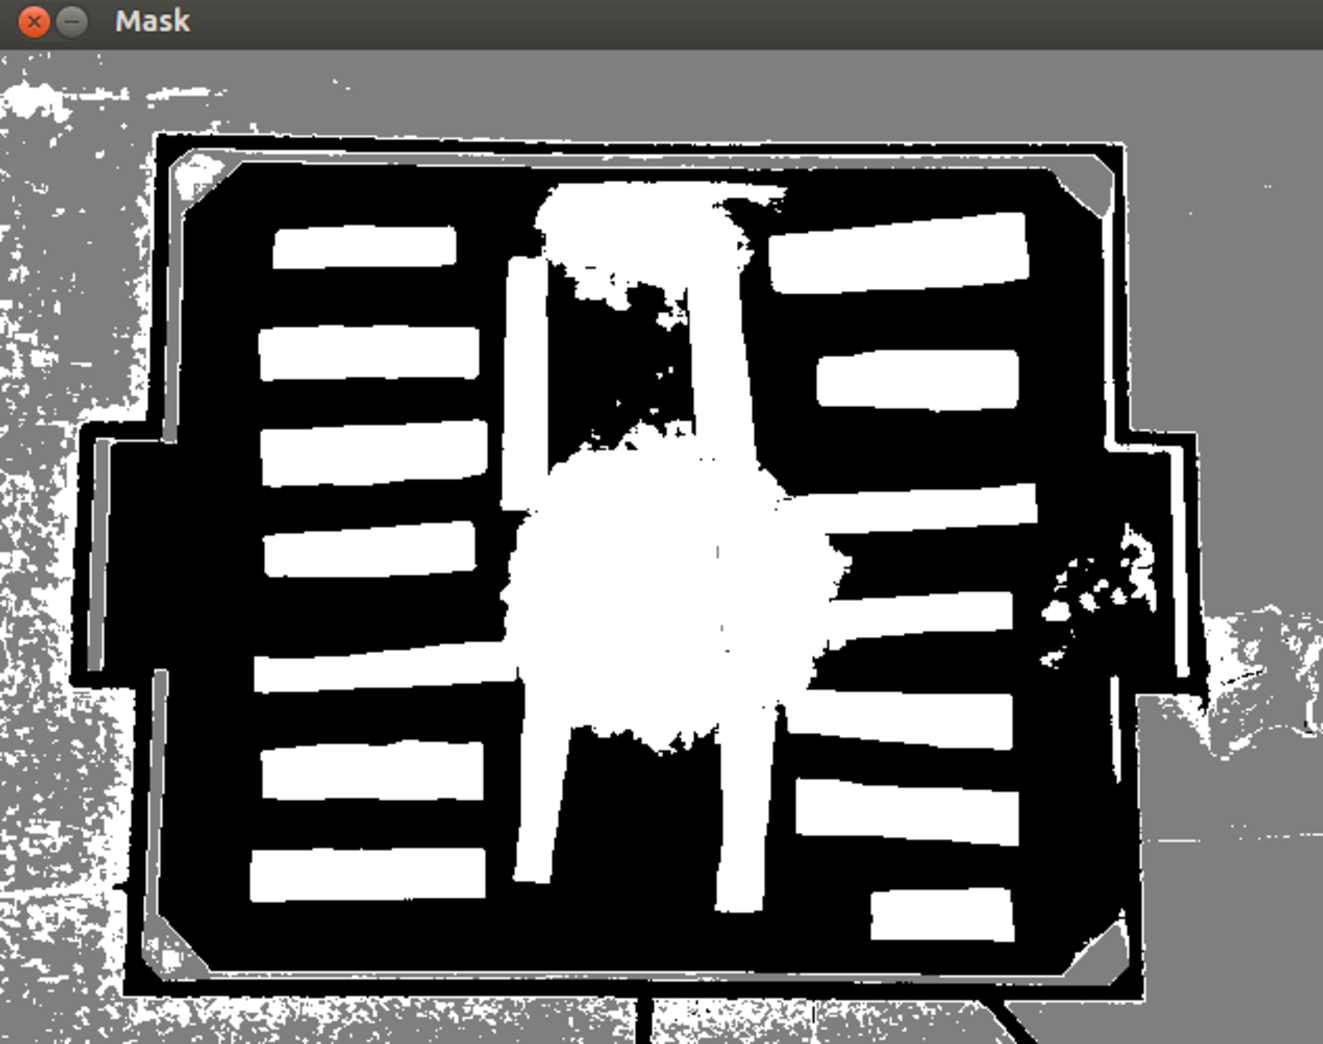
\includegraphics[width=0.6\textwidth]{mascaragerada.pdf}
%		\caption{Objetos dispostos no campo para calibração}
%		\label{disposicaoparte}
%	\end{figure}
	
	\begin{figure}[H]
\begin{minipage}[H]{0.34\linewidth}
\centering
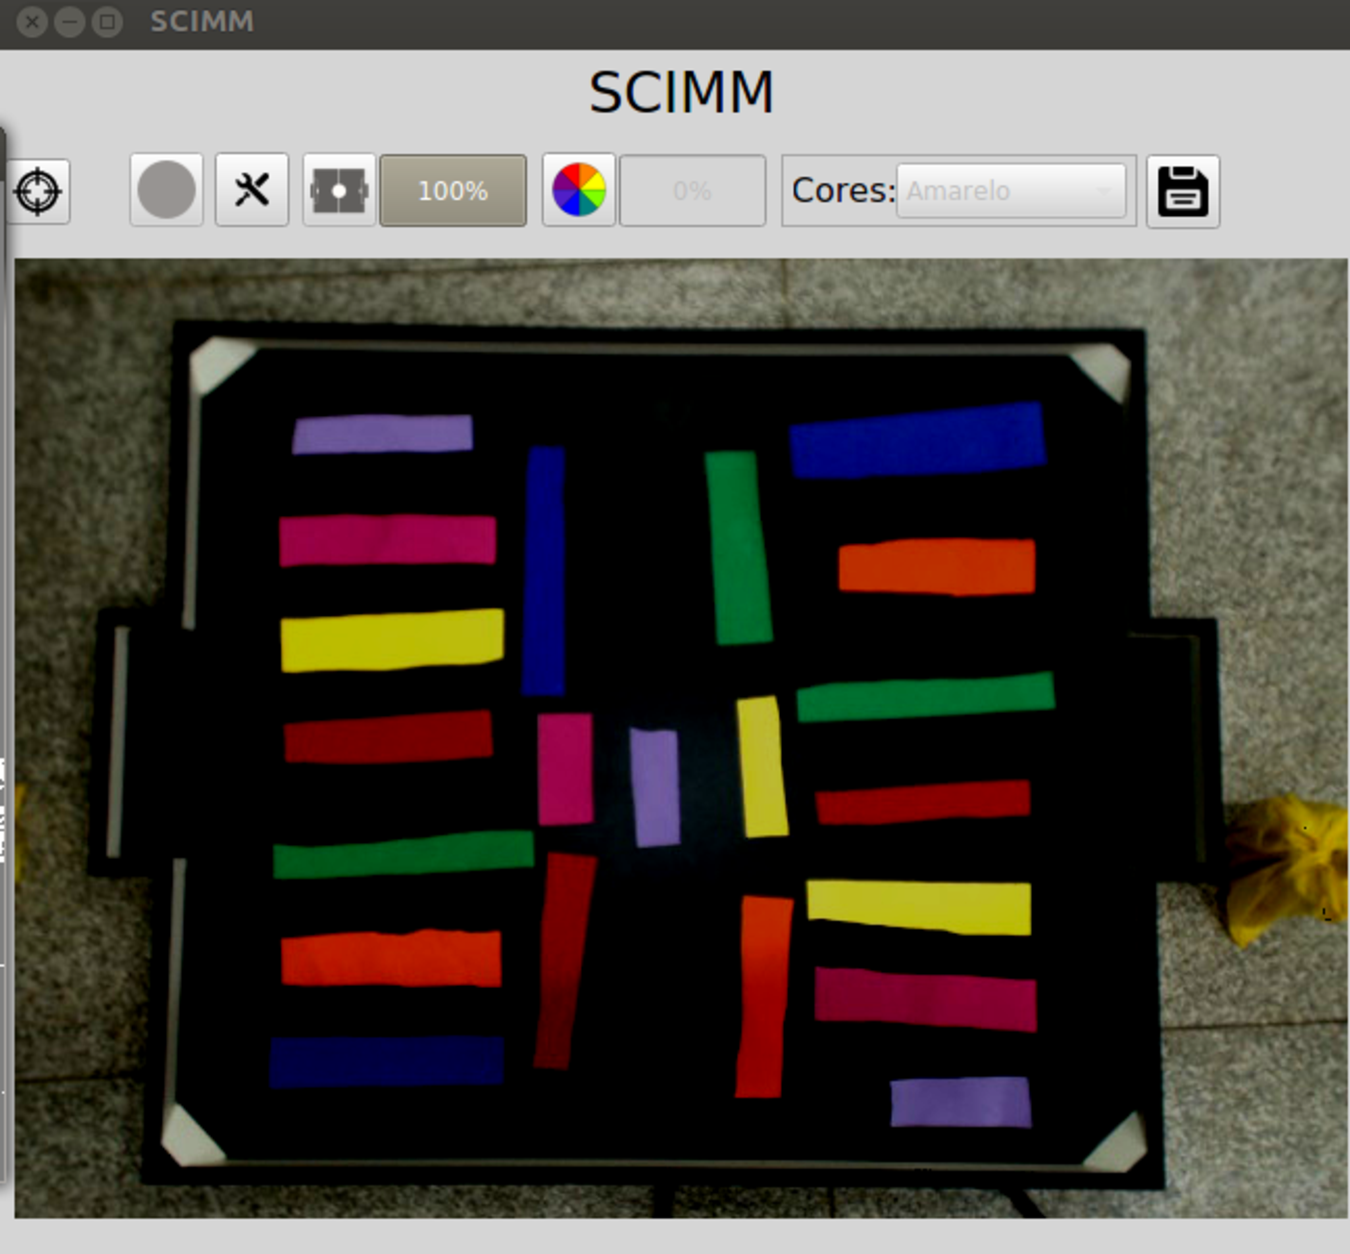
\includegraphics[width=\textwidth]{objetosdispostos.pdf}
\caption{Objetos dispostos no campo para calibração}
\label{fig:figure1}
\end{minipage}
\hspace{0.5cm}
\begin{minipage}[H]{0.40\linewidth}
\centering
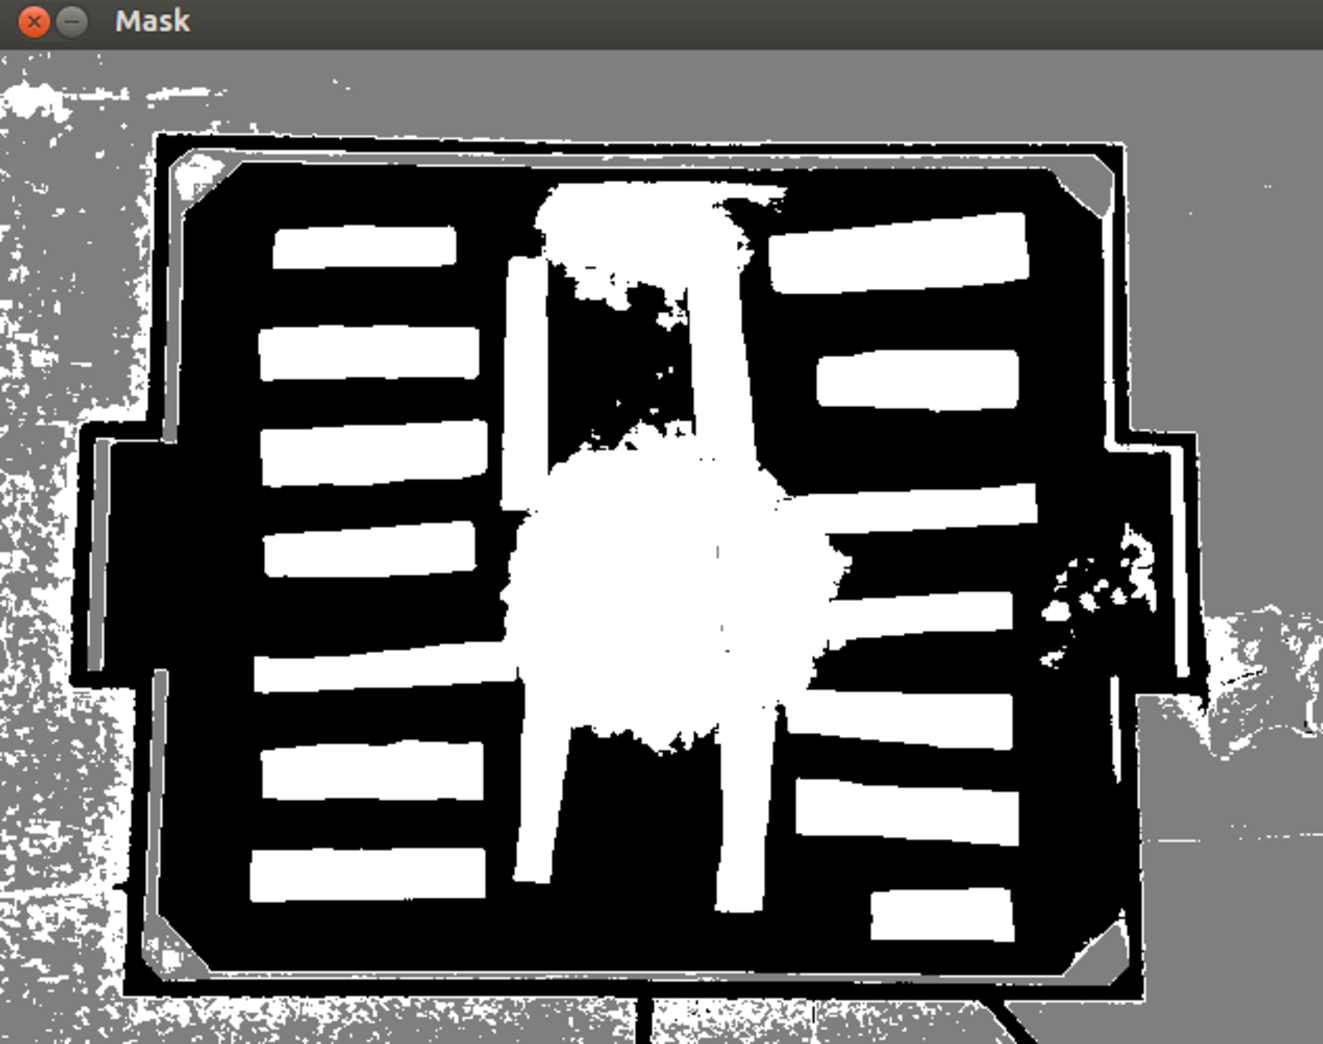
\includegraphics[width=\textwidth]{mascaragerada.pdf}
\caption{Mascara gerada a partir da subtração de fundo}
\label{fig:figure2}
\end{minipage}
\end{figure}	
	
	
Arquivo \textit{cores.arff} gerado:
\begin{center}
21.50.50 \newline
30.255.255\newline
92.100.100\newline
120.255.255\newline
62.100.100\newline
90.255.255\newline
169.100.100\newline
179.255.255\newline
0.100.100\newline
20.255.255\newline
161.100.100\newline
168.255.255\newline
126.30.30\newline
160.255.255\newline
\end{center}
\section{Amarelo}
	\begin{figure}[H]
		\centering
		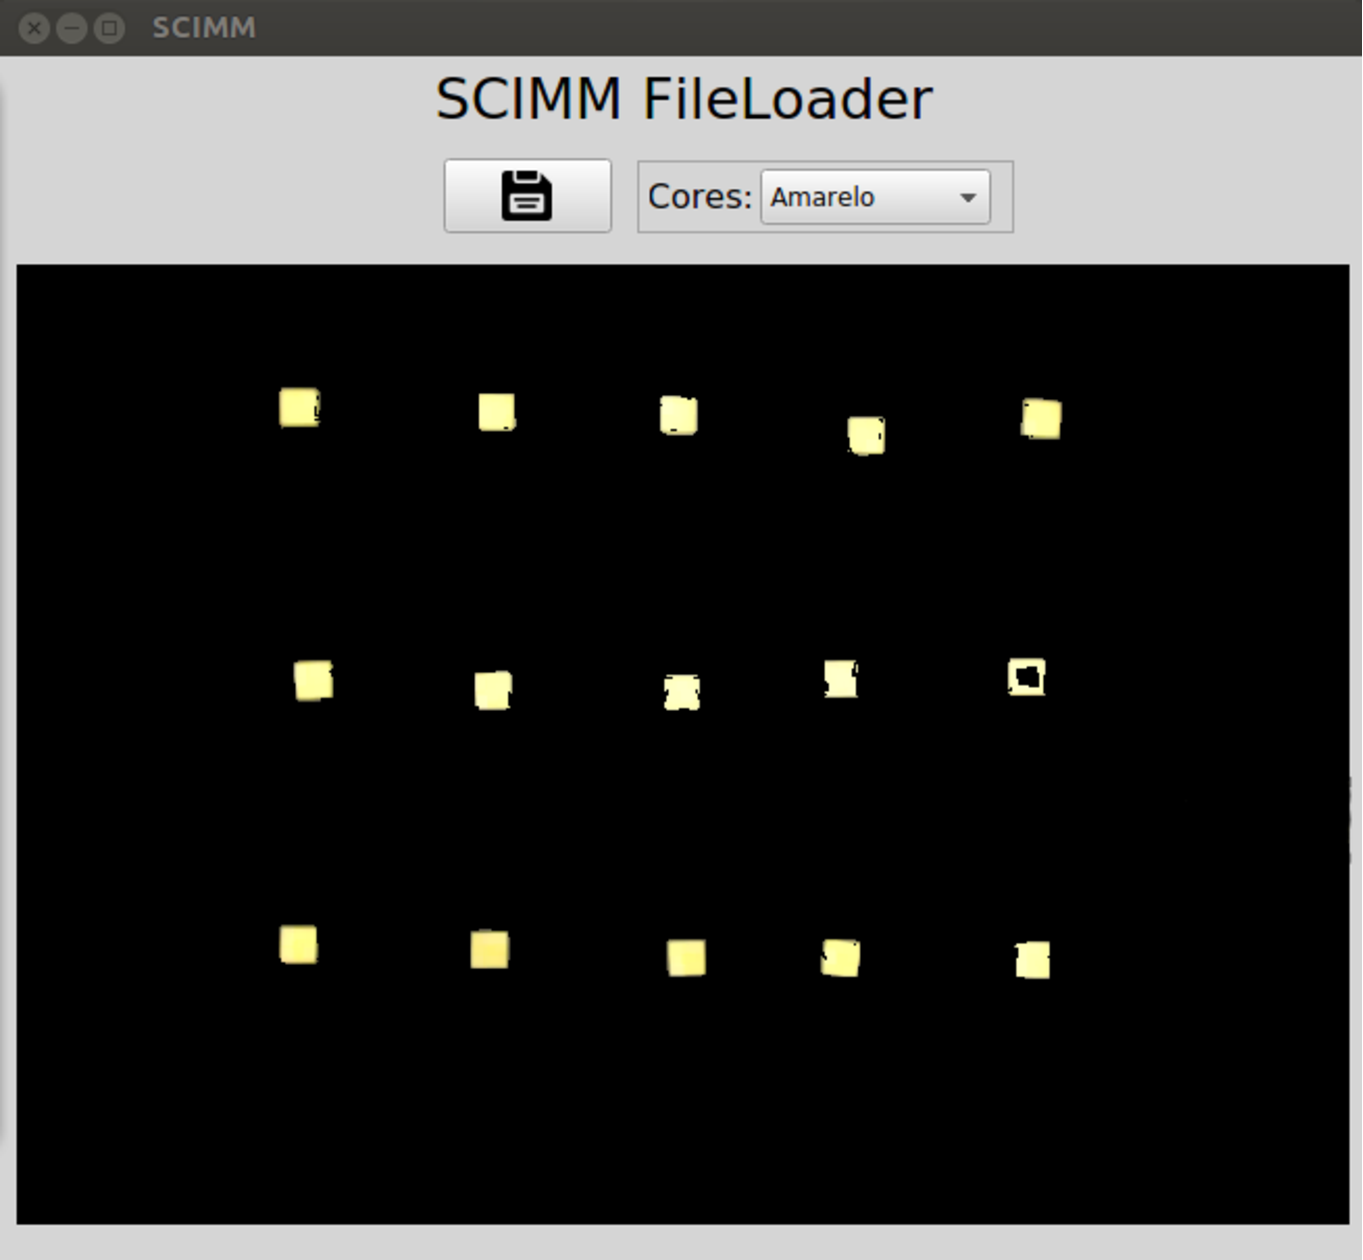
\includegraphics[width=0.5\textwidth]{/testes/amarelo.pdf}
		\caption{Resultado final da cor amarela}
		\label{disposicaoparte}
	\end{figure}
	
	Dentre os objetos da cor amarela o sistema encontrou quatorze deles completamente e apenas um, que devido a luminosidade implicada em seu centro deixando a tonalizadade muito perto do branco, não totalmente preenchido.
\section{Azul}
	\begin{figure}[H]
		\centering
		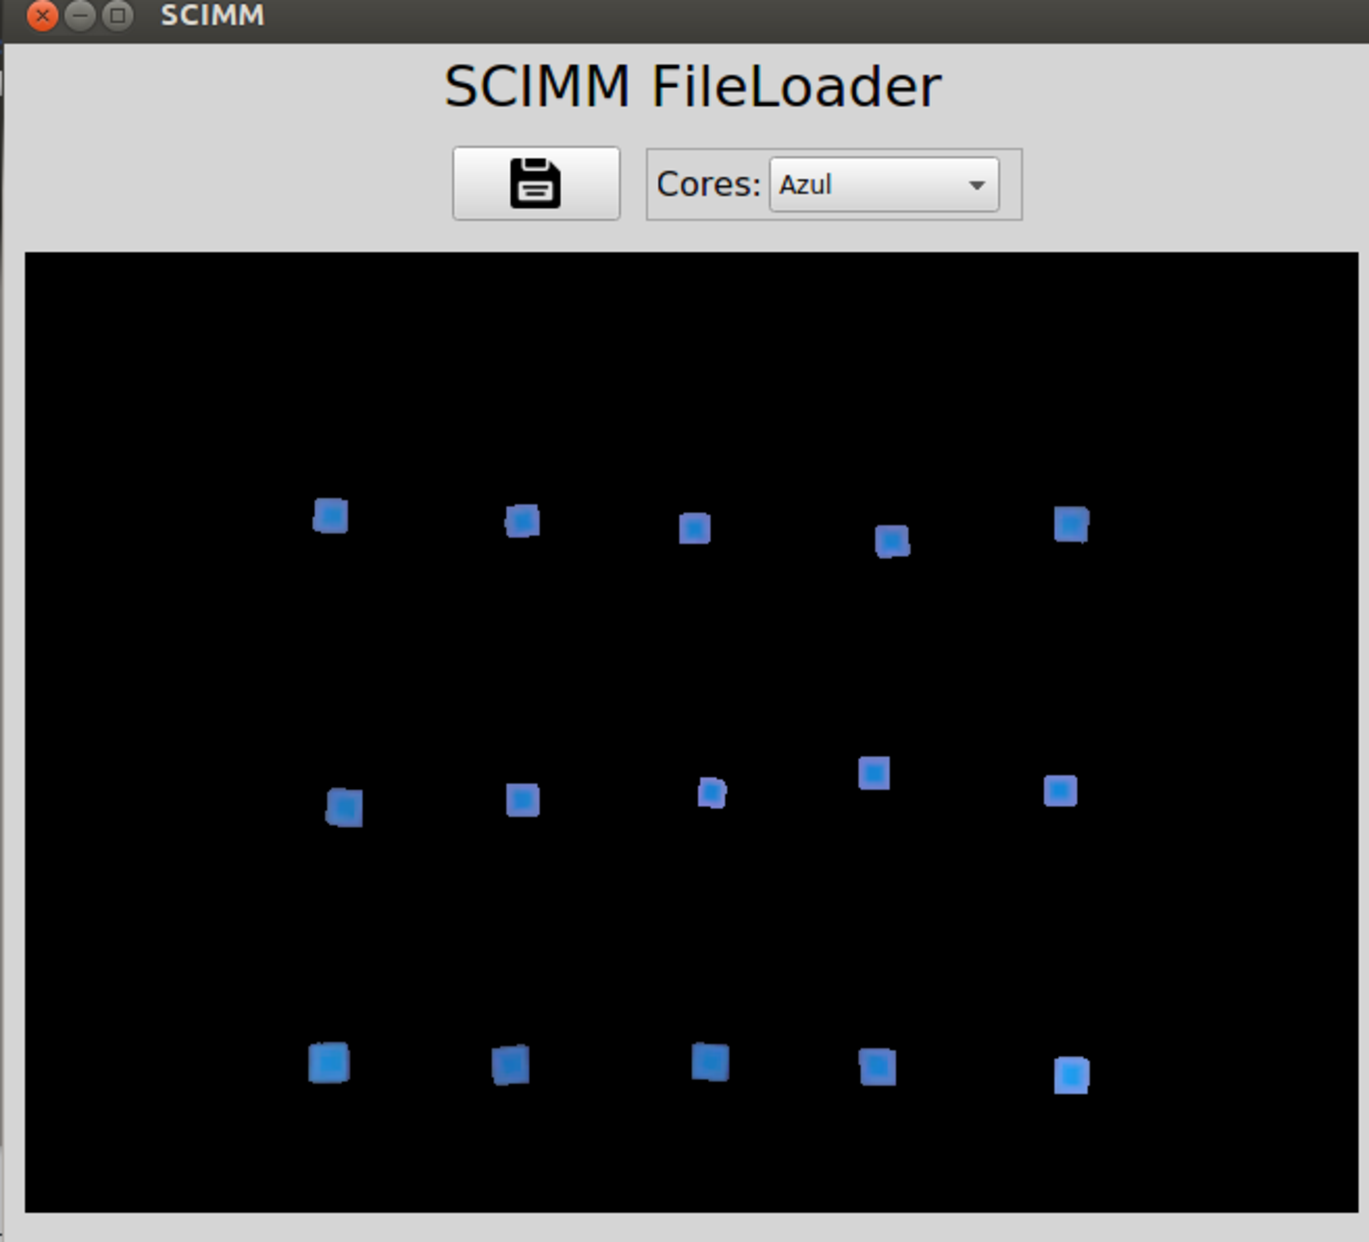
\includegraphics[width=0.5\textwidth]{/testes/azul.pdf}
		\caption{Resultado final da cor amarela}
		\label{disposicaoparte}
	\end{figure}

Os objetos da cor azul foram os que obtiveram os melhores resultados, os quinze objetos foram encontrados de forma preenchida.	Apesar dos quinze estarem totalmente preenchido um dos objetos apresenta um tamanho reduzido aos demais devido a sua borda que não foi totamente detectada.

\section{Verde}
	\begin{figure}[H]
		\centering
		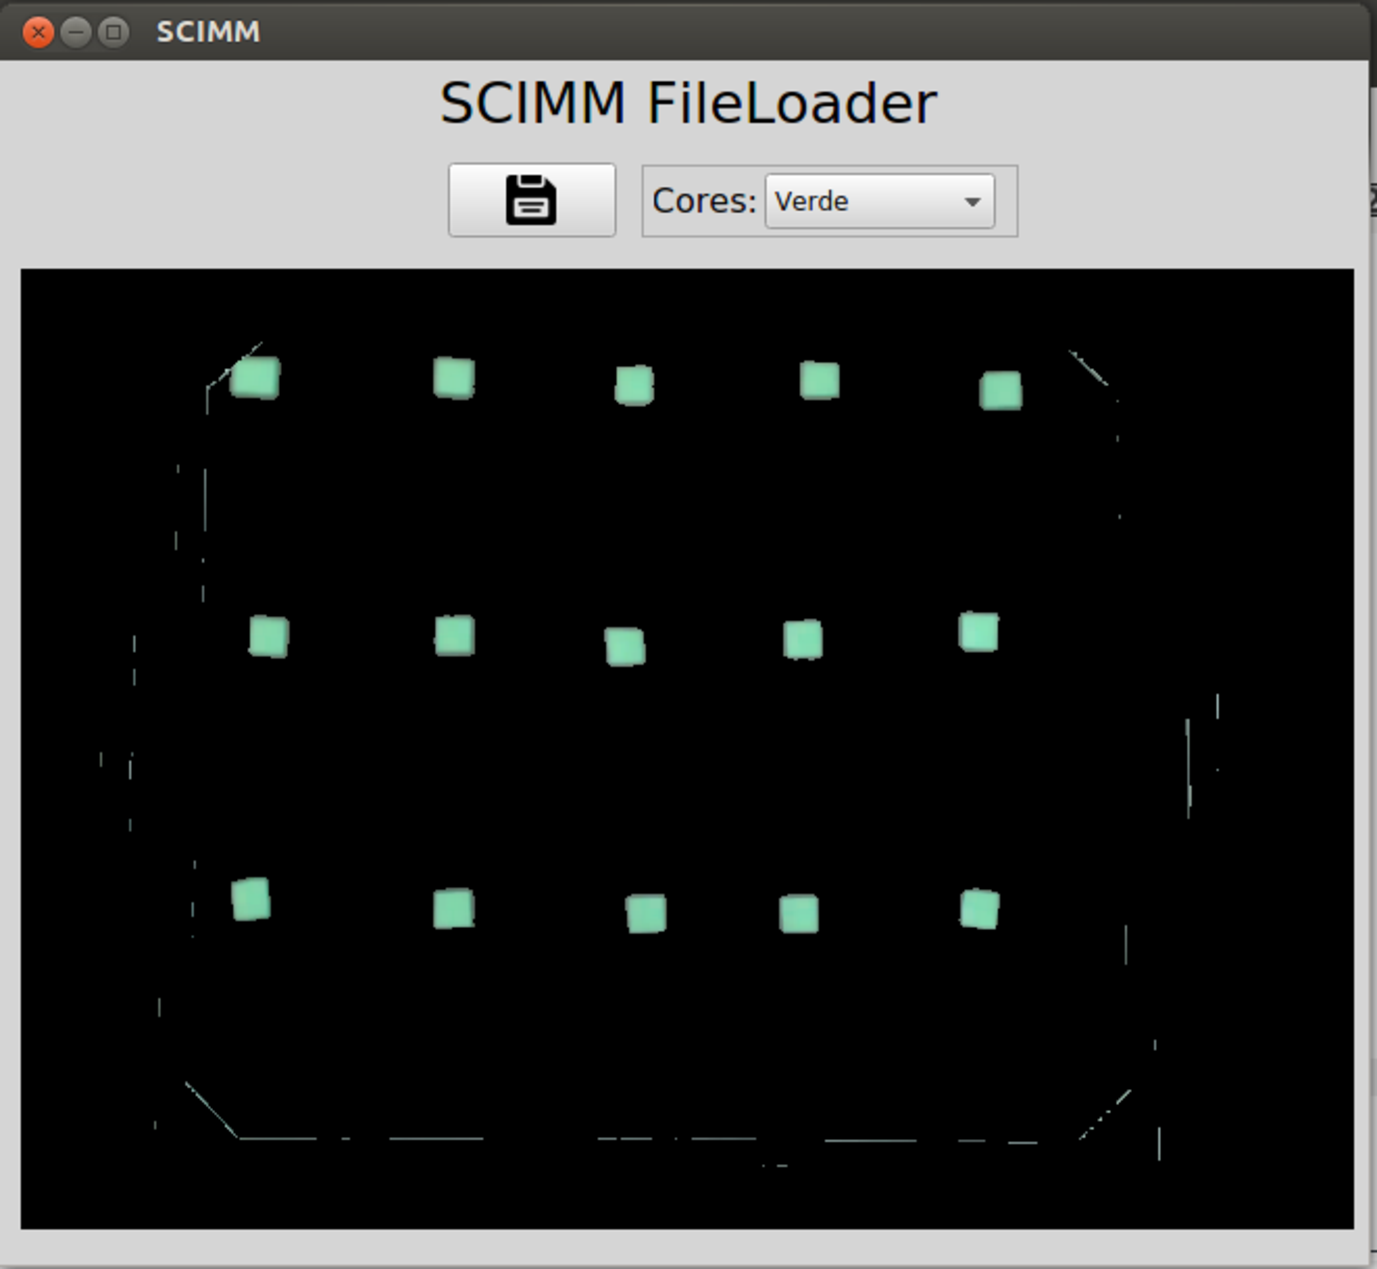
\includegraphics[width=0.5\textwidth]{/testes/verde.pdf}
		\caption{Resultado final da cor verde}
		\label{disposicaoparte}
	\end{figure}

Os objetos da cor verde foram satisfatoriamente encontrados, com seu preenchimento total e sem perca de area devido a qualquer interferencia de luz em sua borda.	
	
\section{Vermelho}
	\begin{figure}[H]
		\centering
		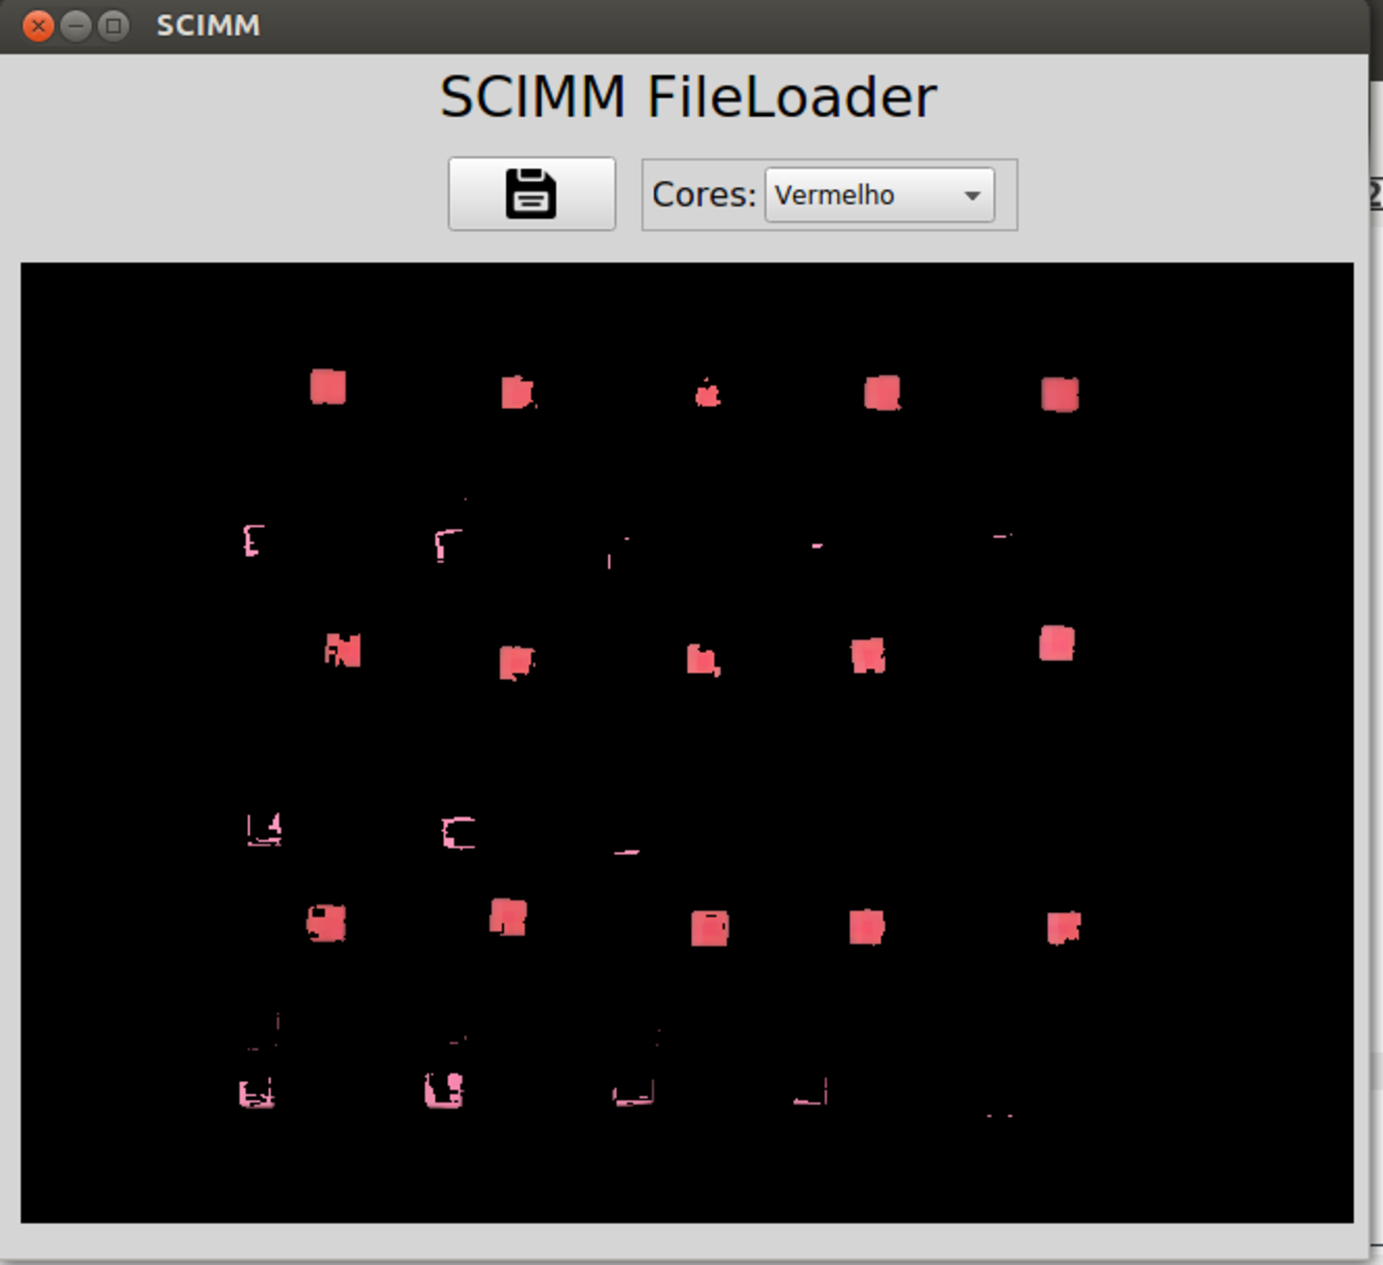
\includegraphics[width=0.5\textwidth]{/testes/vermelho.pdf}
		\caption{Resultado final da cor vermelho}
		\label{disposicaoparte}
	\end{figure}
\section{Rosa}
	\begin{figure}[H]
		\centering
		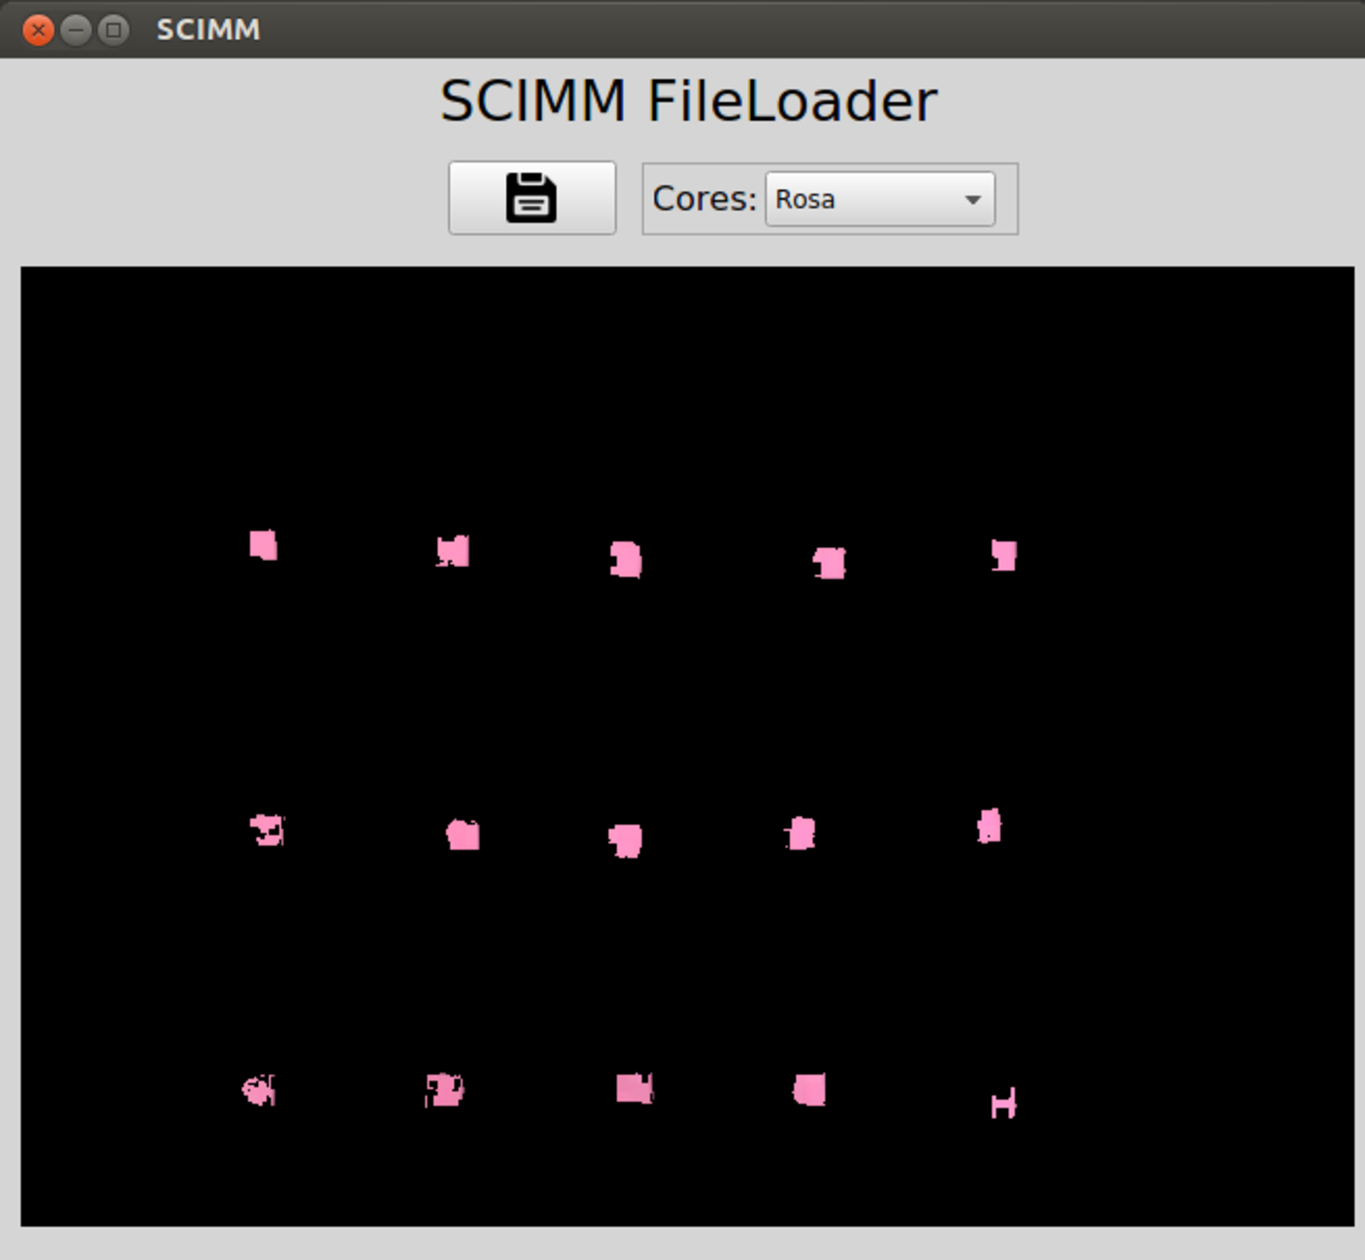
\includegraphics[width=0.5\textwidth]{/testes/rosa.pdf}
		\caption{Resultado final da cor rosa}
		\label{disposicaoparte}
	\end{figure}
\section{Roxo}
	\begin{figure}[H]
		\centering
		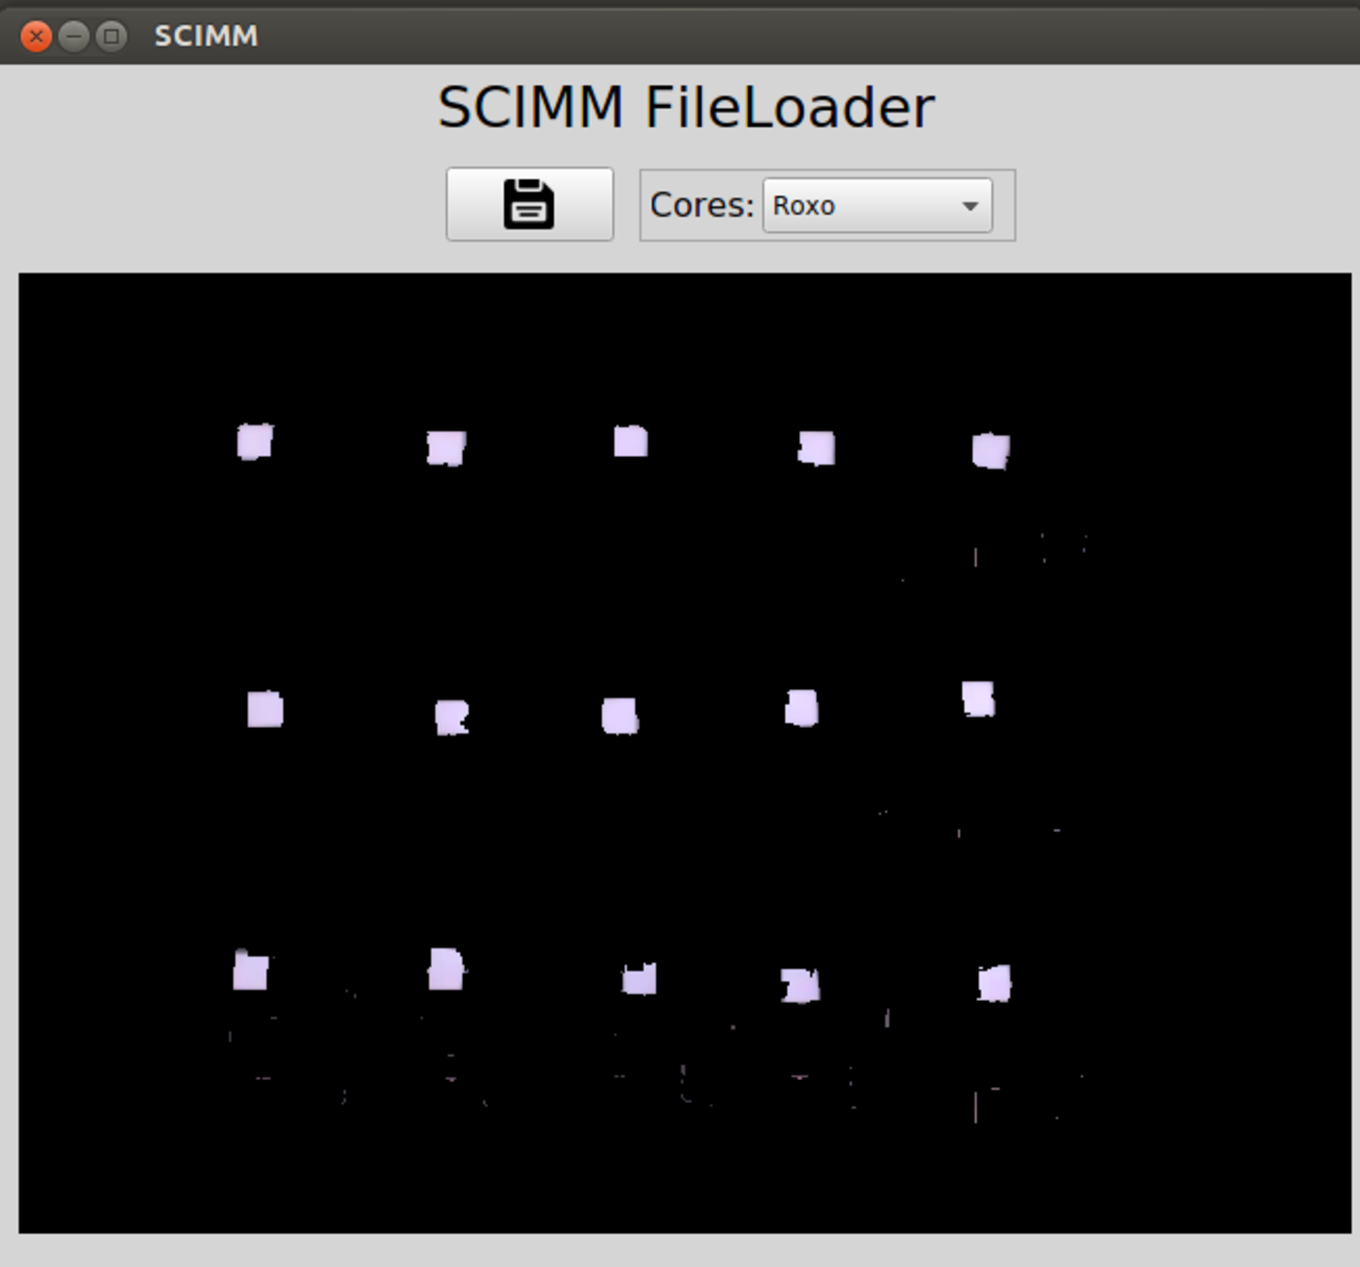
\includegraphics[width=0.5\textwidth]{/testes/roxo.pdf}
		\caption{Resultado final da cor roxo}
		\label{disposicaoparte}
	\end{figure}


	
\section{Laranja}
	\begin{figure}[H]
		\centering
		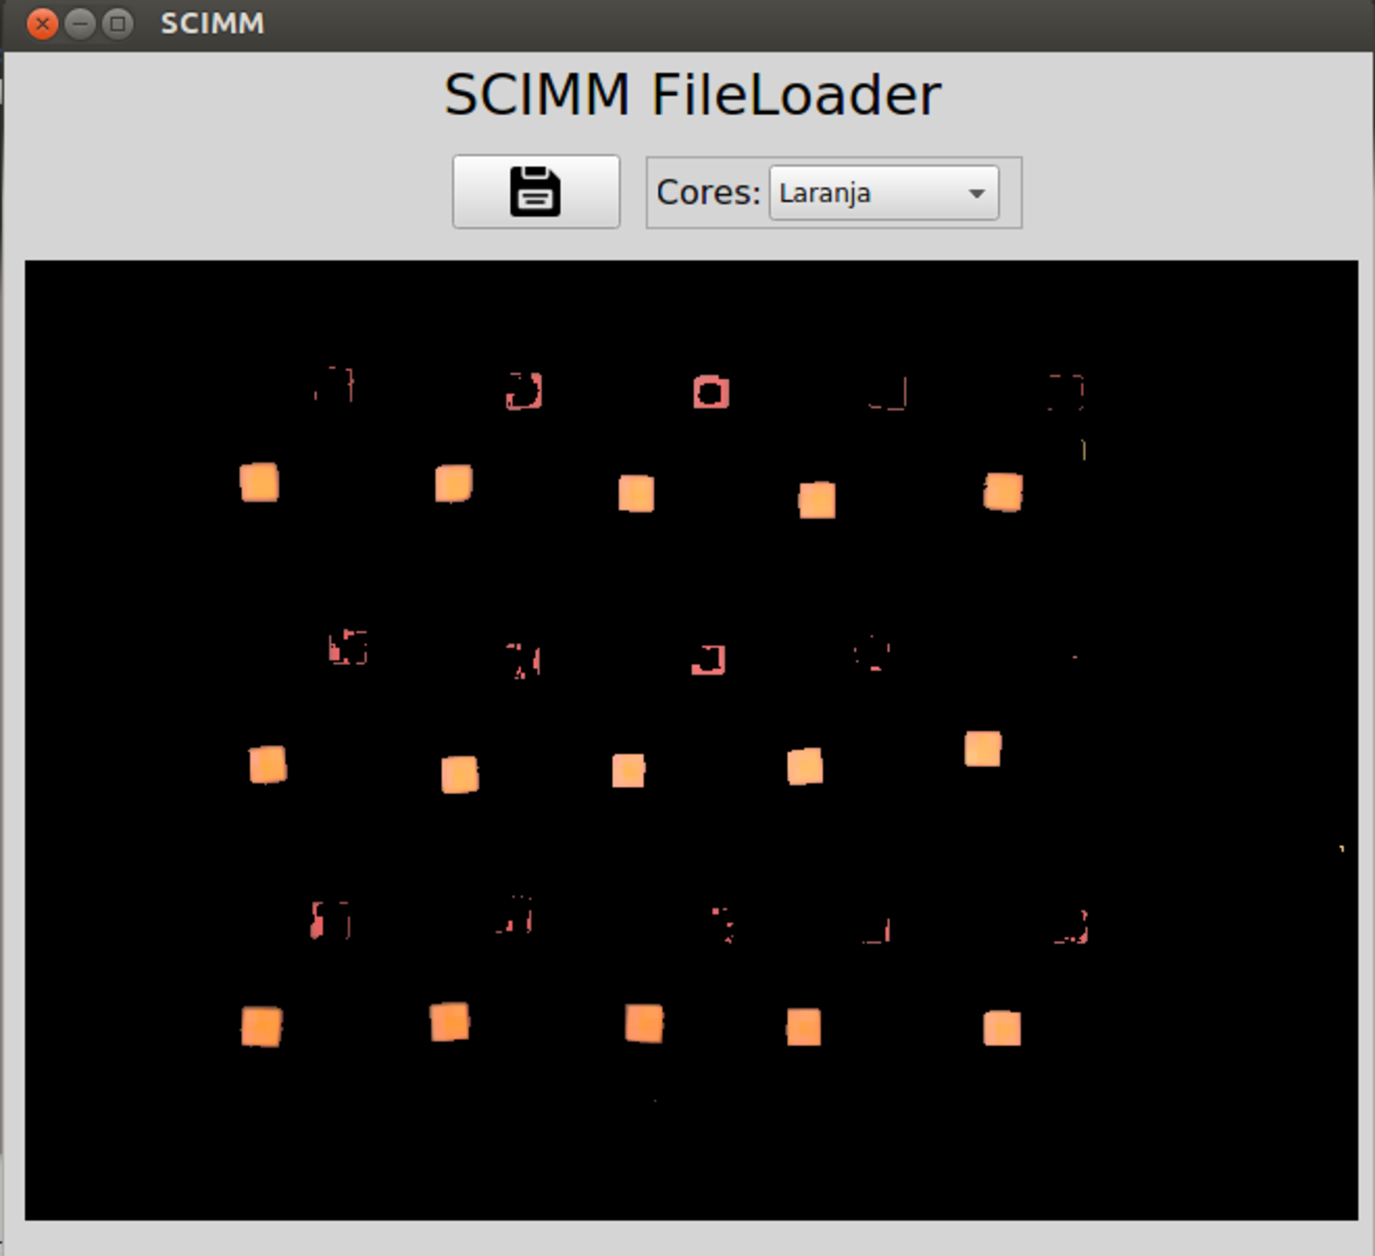
\includegraphics[width=0.5\textwidth]{/testes/laranja.pdf}
		\caption{Resultado final da cor laranja}
		\label{disposicaoparte}
	\end{figure}
	
	Os objetos laranjas foram intencionalmente deixados por ultimo.
	Devido a um problema muito comum na area de calibraçao de cores, a cor laranja possui o problema de ser, por muitas vezes, assemelhada ao vermelho, e devido a luminosidade implicada tanto em uma quanto na outra cor, ambas tendem a se tornarem proximas.
	Sabendo deste problema, o fato de terem sido encontrados objetos da cor vermelha dentro do intervalo de valores da cor laranja é ignorado e somente serão levados em consideração os objetos realmente laranjas.
	Os quinze objetos da cor laranja foram encontrados com precisão. Todos possuindo seu completo preenchimento e borda.
%
%\begin{figure}[H]
%\begin{minipage}[b]{0.30\linewidth}
%\centering
%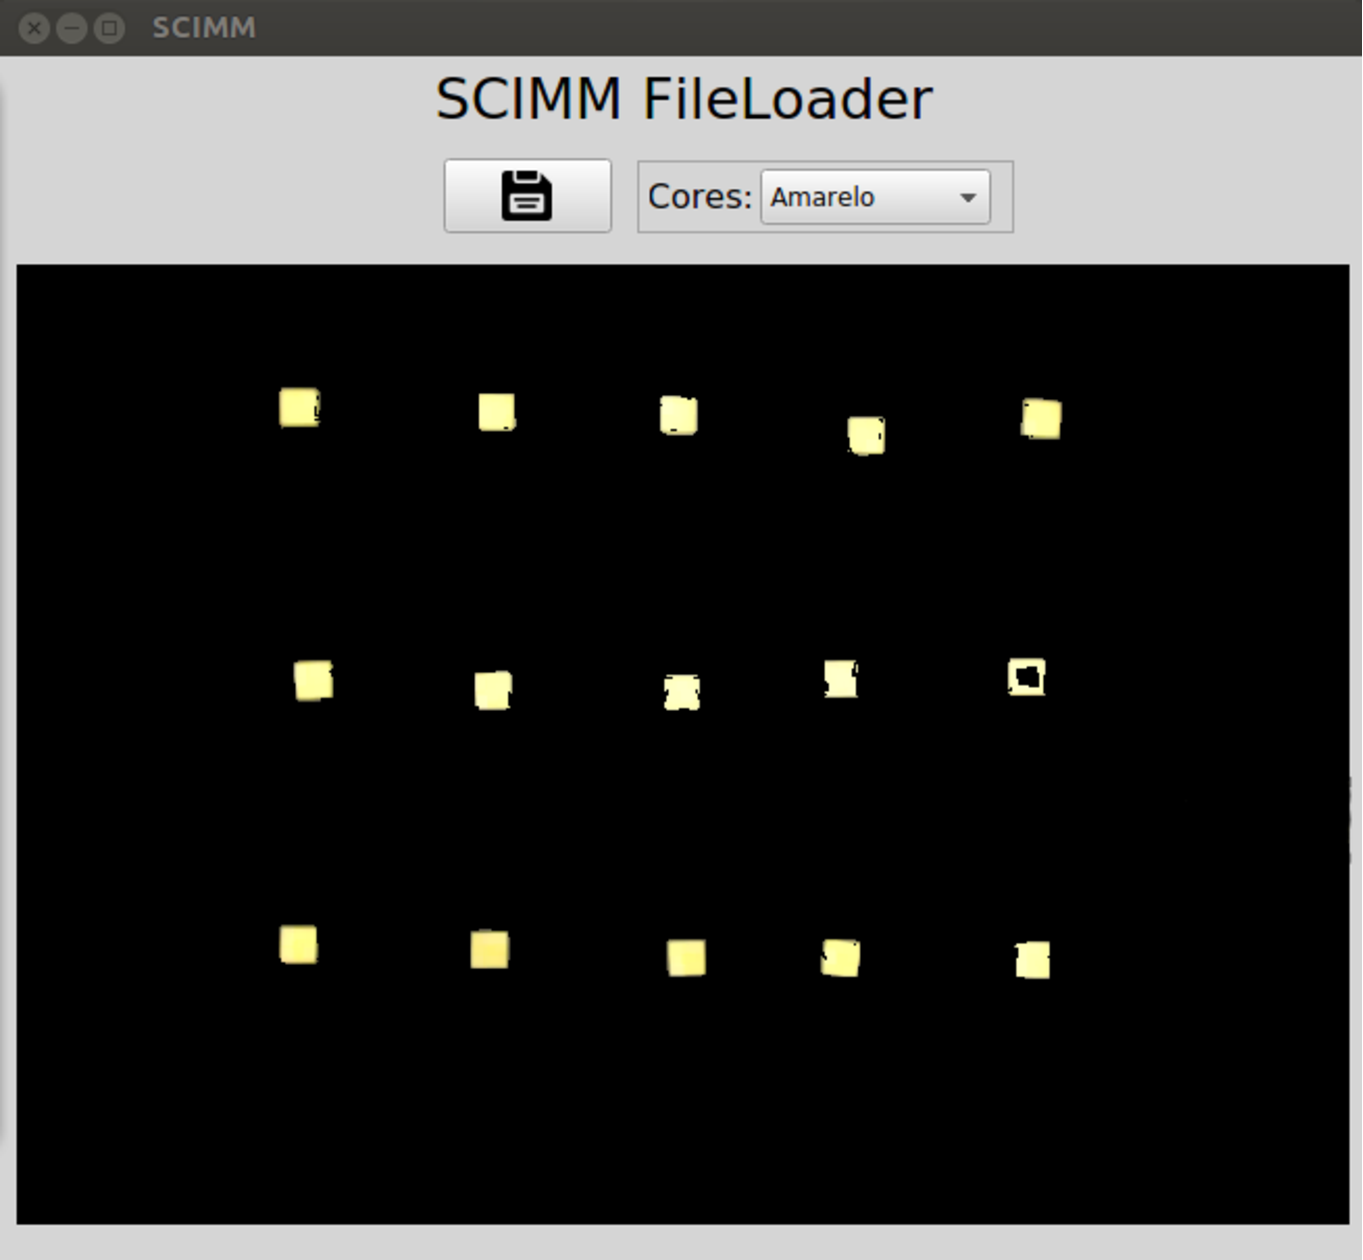
\includegraphics[width=\textwidth]{/testes/amarelo.pdf}
%\caption{Amarelo}
%\label{fig:figure1}
%\end{minipage}
%\hspace{0.5cm}
%\begin{minipage}[b]{0.30\linewidth}
%\centering
%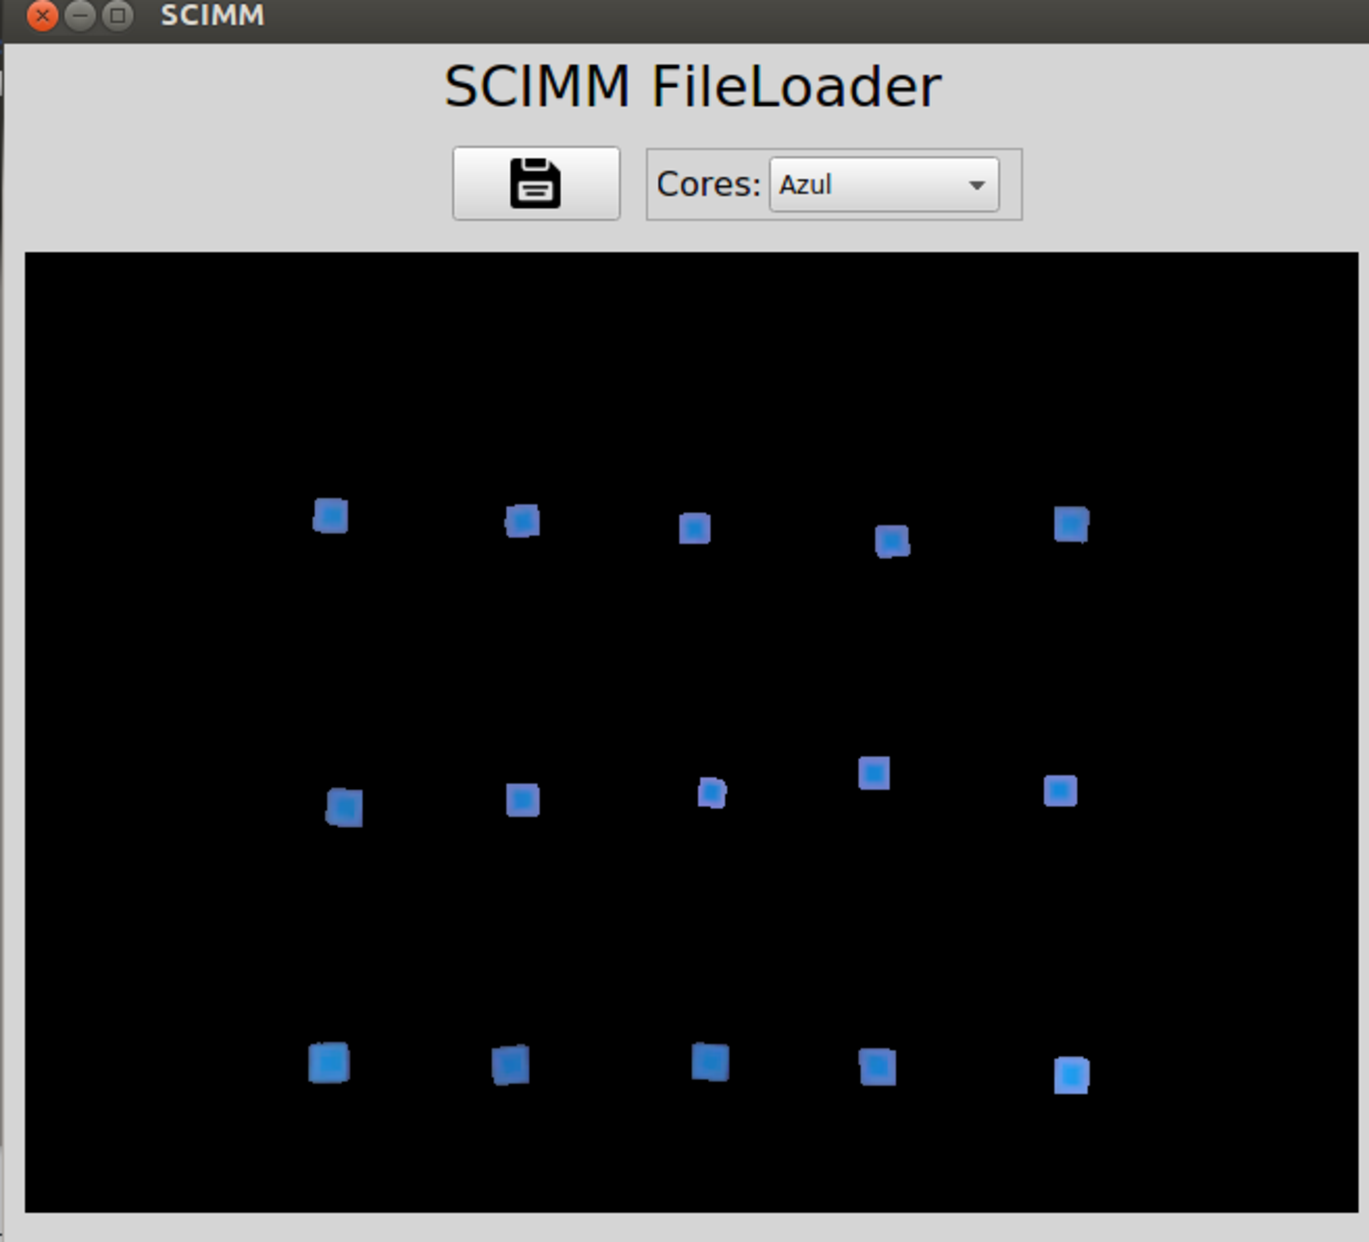
\includegraphics[width=\textwidth]{/testes/azul.pdf}
%\caption{Azul}
%\label{fig:figure2}
%\end{minipage}
%\hspace{0.5cm}
%\begin{minipage}[b]{0.30\linewidth}
%\centering
%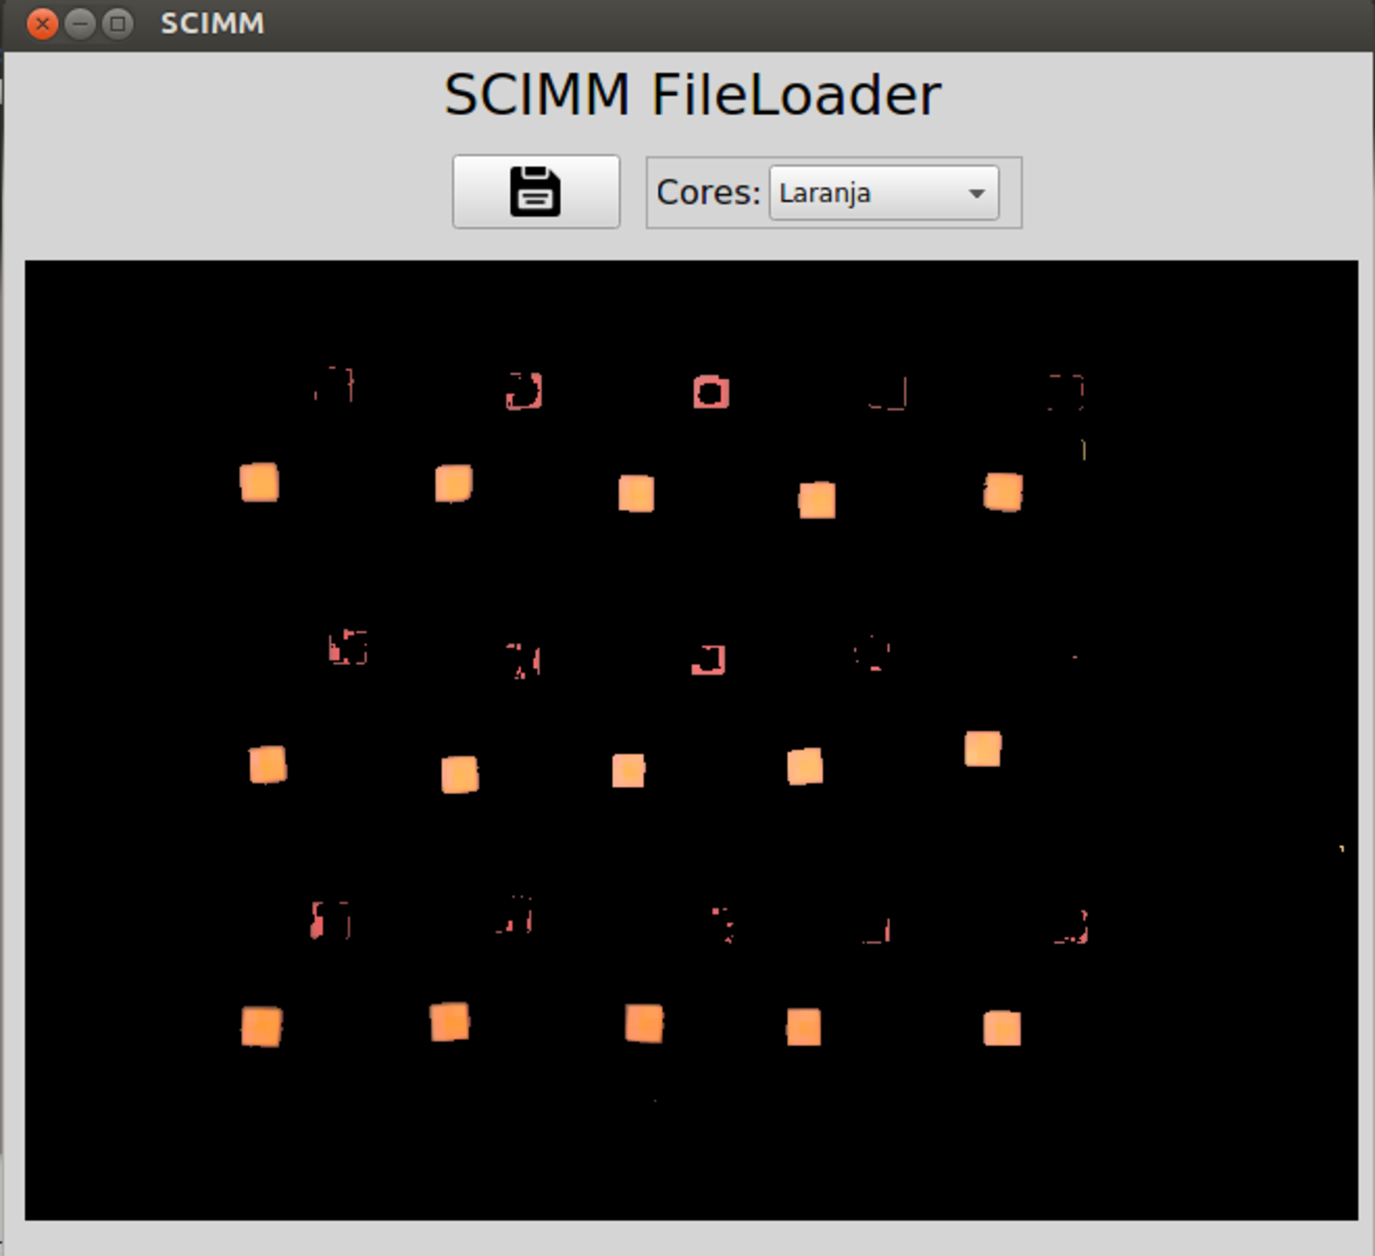
\includegraphics[width=\textwidth]{/testes/laranja.pdf}
%\caption{Laranja}
%\label{fig:figure2}
%\end{minipage}
%\end{figure}
%
%
%	\begin{figure}[H]
%\begin{minipage}[b]{0.30\linewidth}
%\centering
%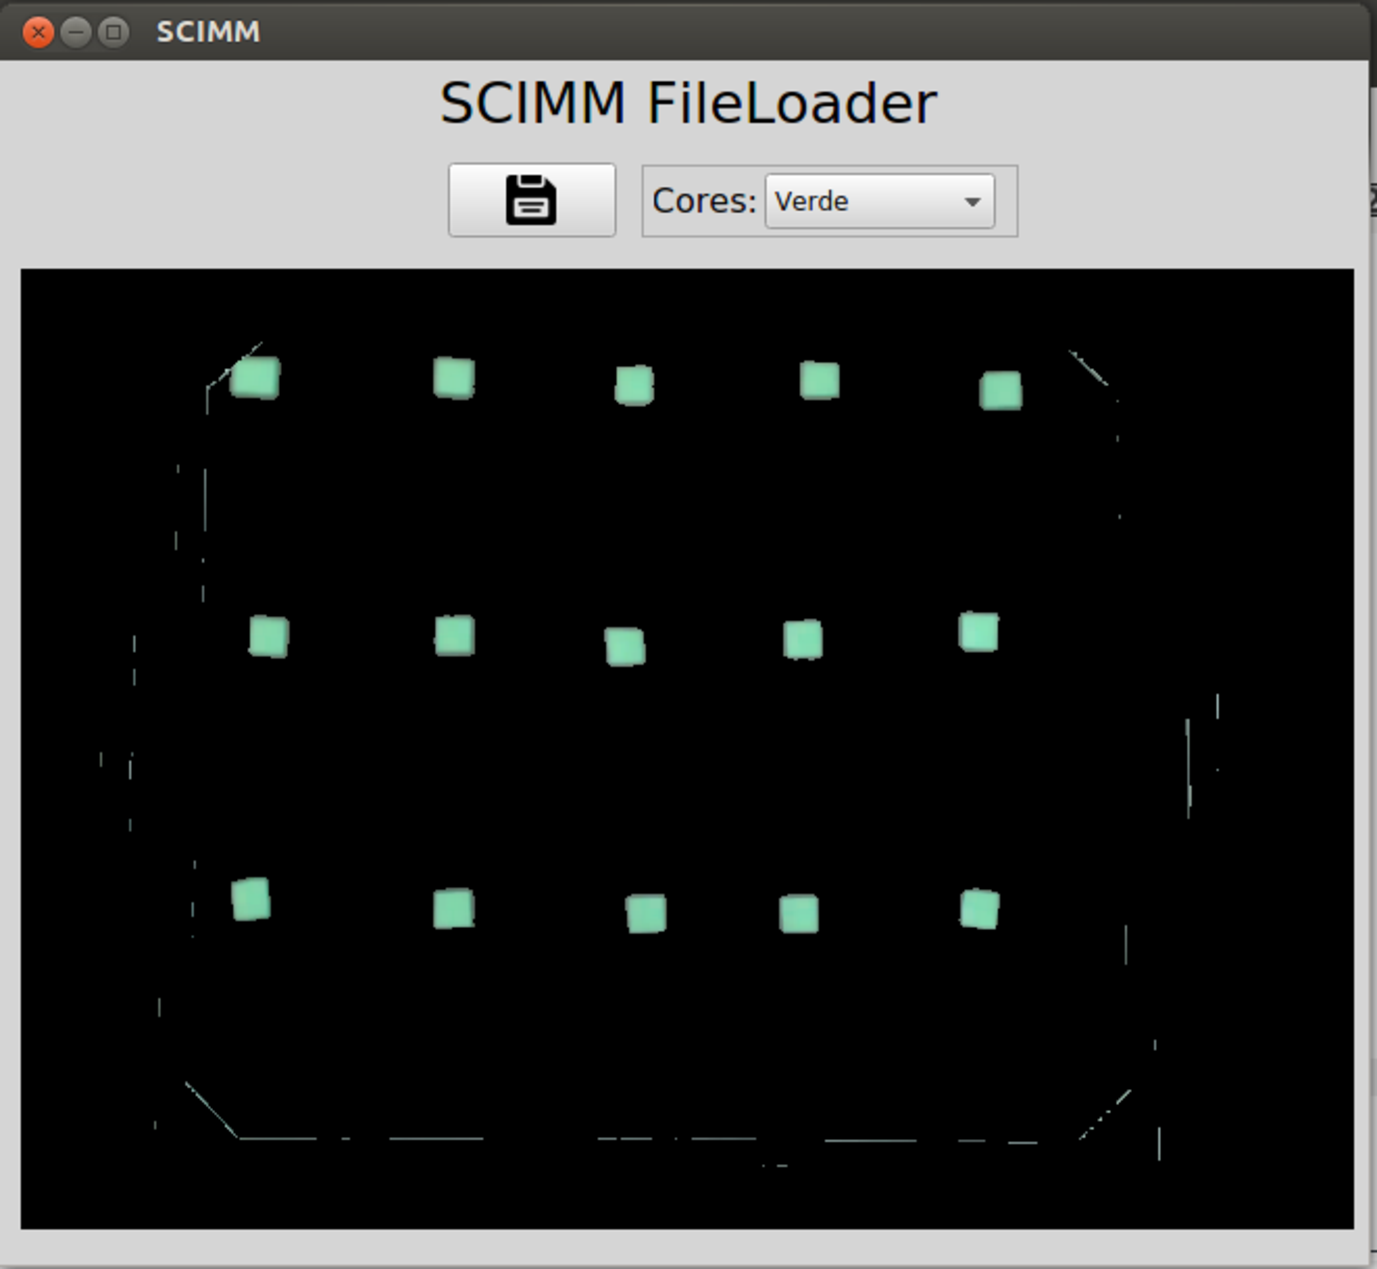
\includegraphics[width=\textwidth]{/testes/verde.pdf}
%\caption{Verde}
%\label{fig:figure1}
%\end{minipage}
%\hspace{0.5cm}
%\begin{minipage}[b]{0.30\linewidth}
%\centering
%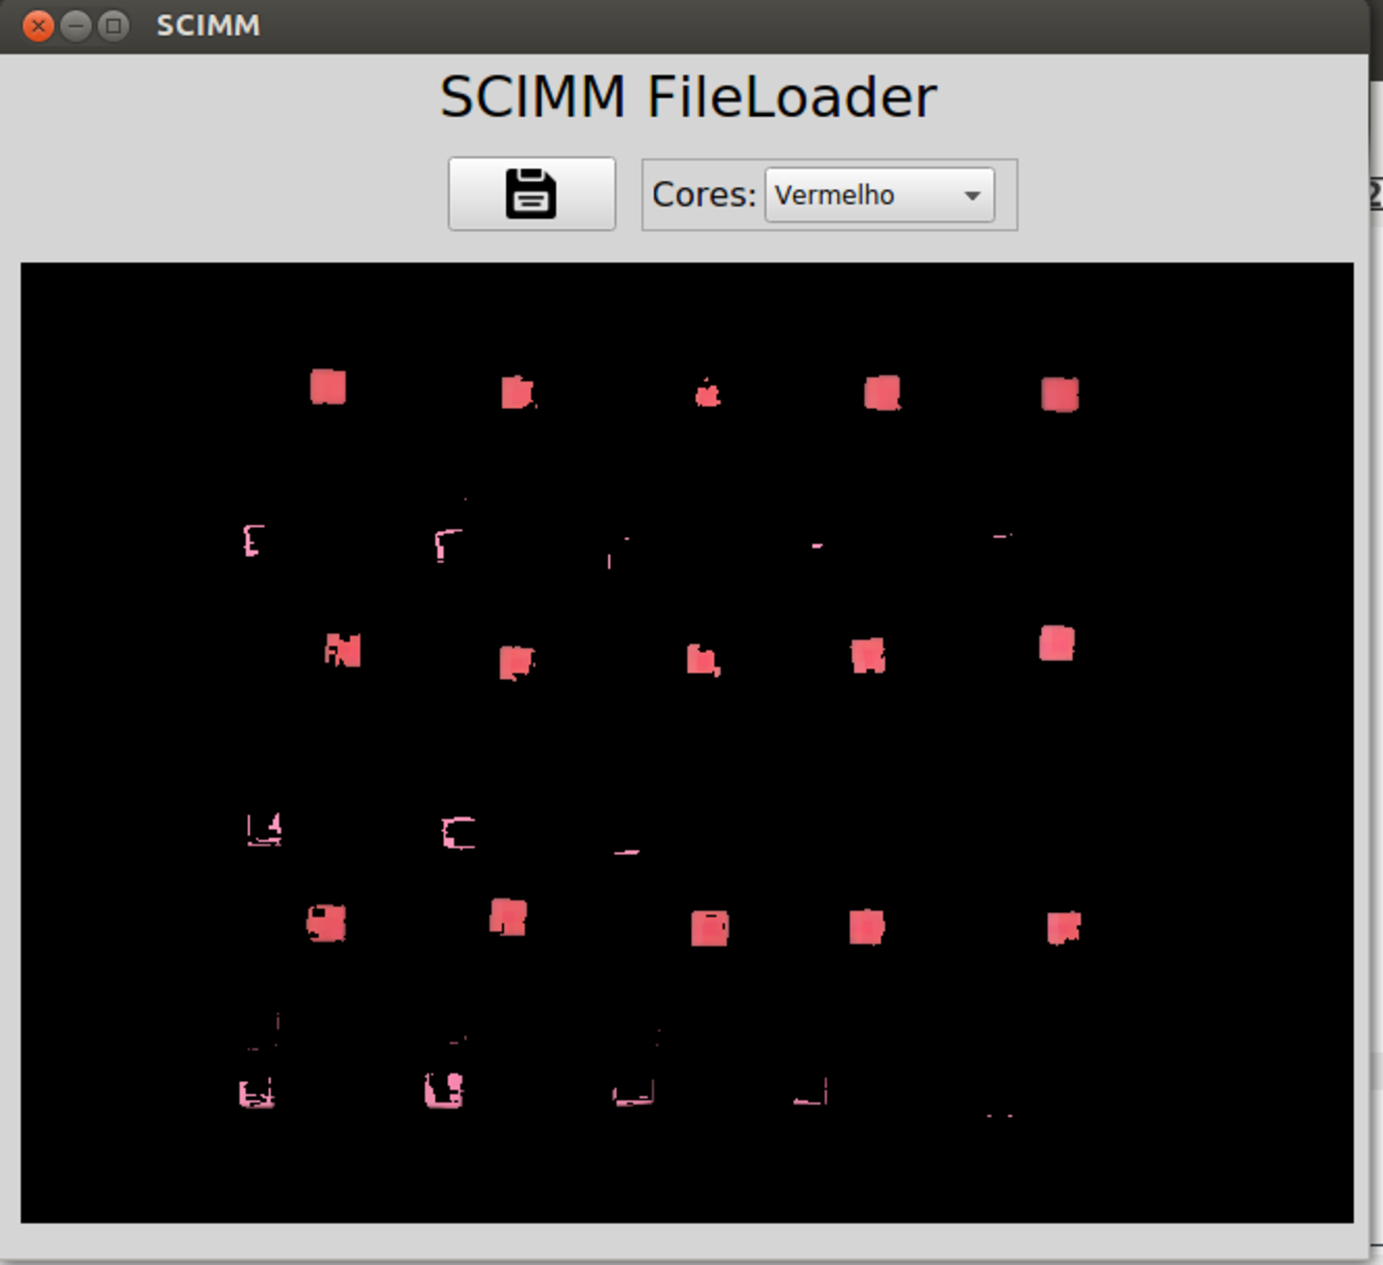
\includegraphics[width=\textwidth]{/testes/vermelho.pdf}
%\caption{Vermelho}
%\label{fig:figure2}
%\end{minipage}
%\hspace{0.5cm}
%\begin{minipage}[b]{0.30\linewidth}
%\centering
%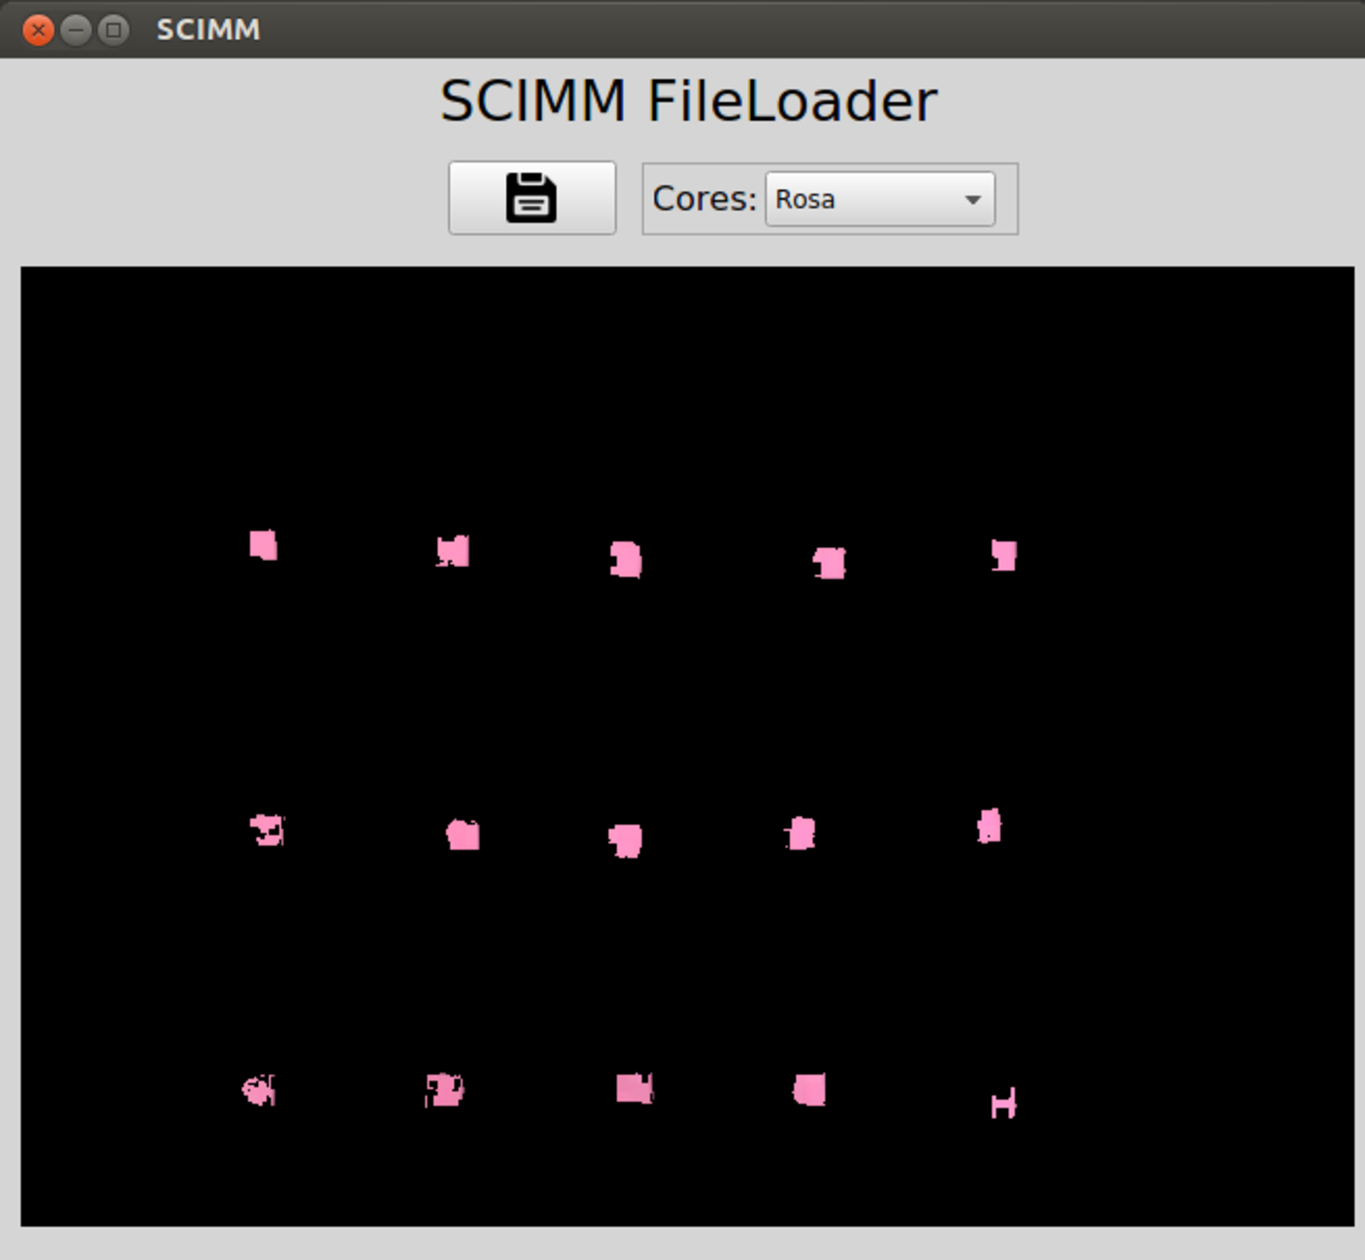
\includegraphics[width=\textwidth]{/testes/rosa.pdf}
%\caption{Rosa}
%\label{fig:figure2}
%\end{minipage}
%\end{figure}
%
%\begin{figure}[H]
%		\centering
%		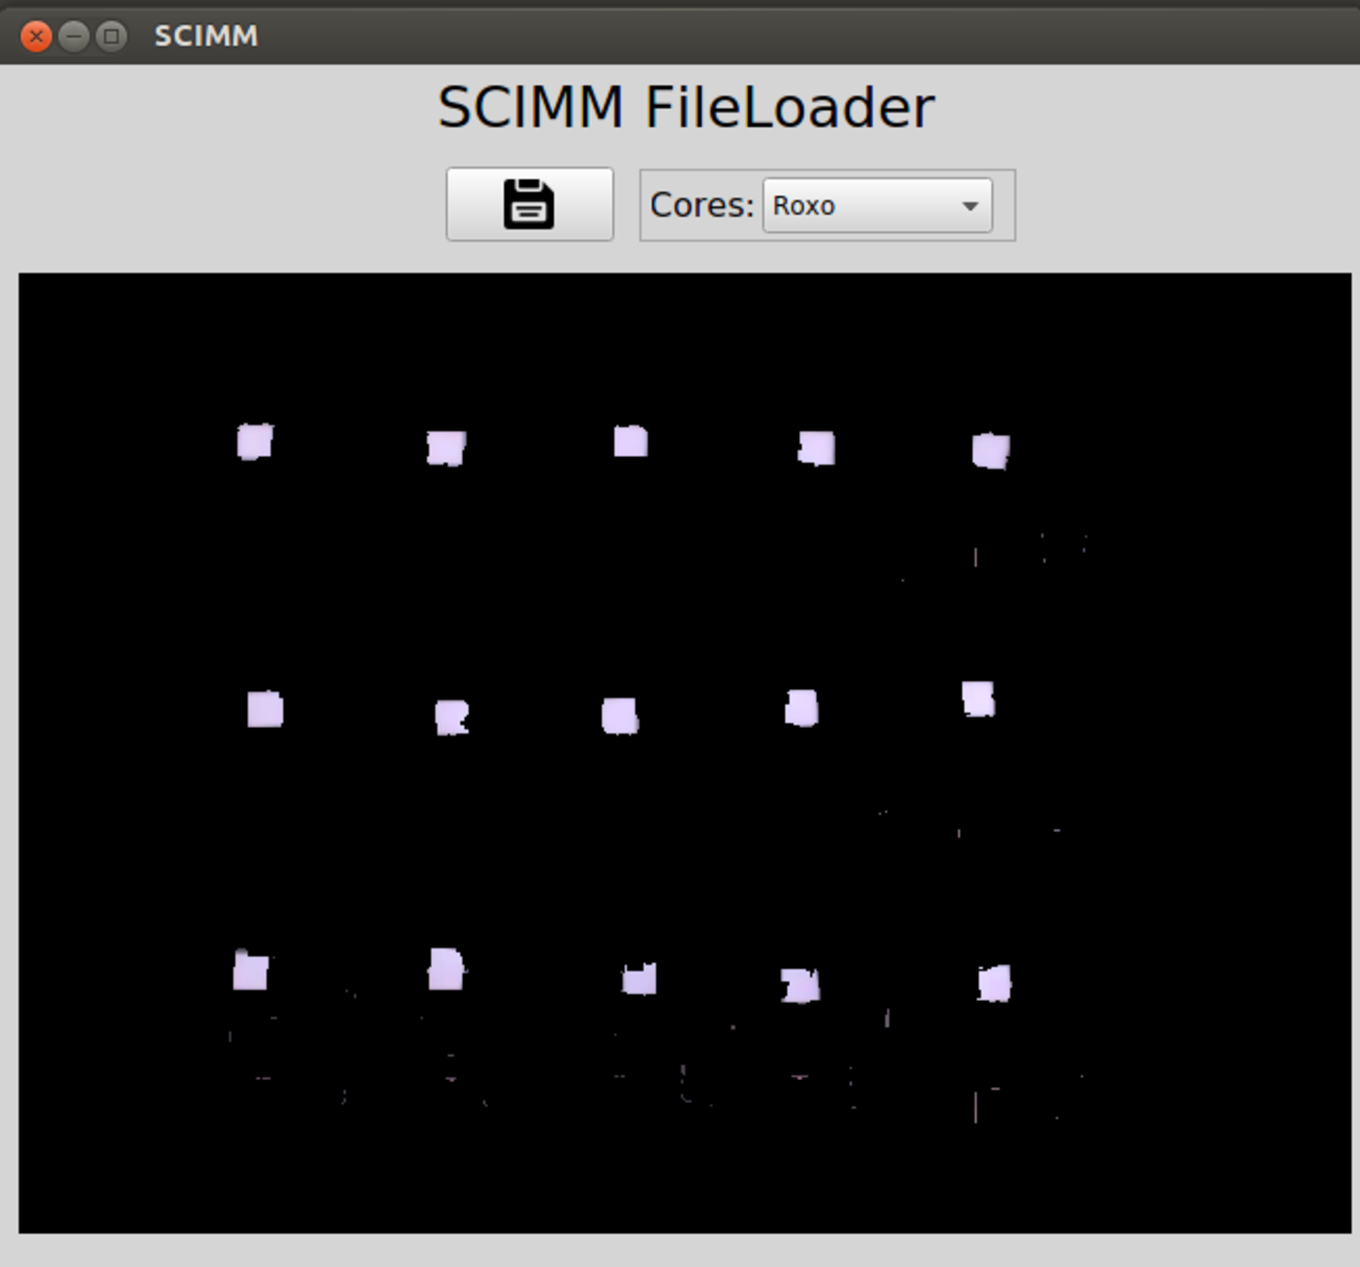
\includegraphics[width=0.3\textwidth]{/testes/roxo.pdf}
%		\caption{Roxos}
%		\label{disposicaoparte}
%	\end{figure}